% =====================================================================
% Internship defense — Vadim Lagresle — Criteo AI Lab — September 2026
% Stabilizing and improving the efficiency of autonomous training for LLM agents
%
% V3 (2026-09-16): redesign following the new six-part plan. Same style as V2.
% Compilation: pdfLaTeX (Overleaf). Figures expected in figures/
% (copy docs/rapport/figures/*.pdf into a figures/ folder of the project).
% Palette inspired by the Criteo brand: orange FE5000, anthracite 2A2E33,
% blue 006CD6, light grey F2F2F0. Font: Fira Sans (close to Graphik).
% =====================================================================
\documentclass[aspectratio=169,10pt]{beamer}
\usepackage[utf8]{inputenc}
\usepackage[T1]{fontenc}
\usepackage[english]{babel}
\usepackage[sfdefault,light]{FiraSans}
\usepackage{amsmath,amssymb}
\usepackage{booktabs}
\usepackage{graphicx}
\usepackage{xcolor}
\usepackage{colortbl}
\usepackage{tikz}
\usetikzlibrary{positioning,arrows.meta,calc}
\usepackage{appendixnumberbeamer}
\graphicspath{{figures/}{../rapport/figures/}}

% ---------- Palette ----------
\definecolor{crOrange}{HTML}{FE5000}
\definecolor{crDark}{HTML}{2A2E33}
\definecolor{crBlue}{HTML}{006CD6}
\definecolor{crGrey}{HTML}{F2F2F0}
\definecolor{crMid}{HTML}{8A8F96}

% ---------- Theme ----------
\usetheme{default}
\usecolortheme{seagull}
\setbeamertemplate{navigation symbols}{}
\setbeamercolor{normal text}{fg=crDark,bg=white}
\setbeamercolor{structure}{fg=crOrange}
\setbeamercolor{alerted text}{fg=crOrange}
\setbeamercolor{frametitle}{fg=crDark,bg=white}
\setbeamerfont{frametitle}{size=\Large,series=\bfseries}
\setbeamercolor{block title}{fg=white,bg=crOrange}
\setbeamercolor{block body}{fg=crDark,bg=crGrey}
\setbeamerfont{block title}{series=\bfseries}
\setbeamercolor{item}{fg=crOrange}
\setbeamertemplate{itemize items}{\raisebox{0.15ex}{\tikz\fill[crOrange] (0,0) rectangle (0.5ex,0.5ex);}}
\setbeamertemplate{enumerate items}[default]
\setbeamercolor{enumerate item}{fg=crOrange}
\setbeamercolor{caption name}{fg=crMid}
\setbeamertemplate{blocks}[rounded=false]

% Slide title: anthracite text + short orange rule underneath
\setbeamertemplate{frametitle}{%
  \vspace{0.3cm}%
  \begin{minipage}{\dimexpr\textwidth}
    \usebeamerfont{frametitle}\usebeamercolor[fg]{frametitle}\insertframetitle\par
    \vspace{0.08cm}\textcolor{crOrange}{\rule{1.6cm}{2.2pt}}
  \end{minipage}\vspace{0.05cm}}

% Footer: thin line, name, short title, page number
\setbeamertemplate{footline}{%
  \vbox{%
    \hbox to \paperwidth{\hskip0.9cm\textcolor{crOrange}{\rule{\dimexpr\paperwidth-1.8cm\relax}{0.6pt}}\hfil}%
    \vskip 3pt
    \hbox to \paperwidth{\hskip0.9cm{\scriptsize\textcolor{crMid}{Vadim Lagresle \;·\; Stabilizing and improving the efficiency of autonomous training for LLM agents \;·\; Criteo AI Lab}}\hfil{\scriptsize\textcolor{crMid}{\insertframenumber}}\hskip0.9cm}%
    \vskip 5pt}}

% Section pages: orange background, white text
\newif\ifinappendix
\AtBeginSection[]{%
  \begingroup
  \setbeamercolor{background canvas}{bg=crOrange}
  \setbeamertemplate{footline}{}
  \begin{frame}[plain]
    \vfill
    \begin{minipage}{0.85\textwidth}
      {\color{white}\scriptsize\bfseries \ifinappendix APPENDIX\else PART \thesection\fi}\\[0.3cm]
      {\color{white}\huge\bfseries\insertsectionhead}\\[0.4cm]
      {\color{white}\rule{2.4cm}{2.5pt}}
    \end{minipage}
    \vfill
  \end{frame}
  \endgroup}

% ---------- Macros ----------
\newcommand{\refs}[1]{\vfill{\tiny\textcolor{crMid}{Refs: #1}}}
\newcommand{\kpi}[2]{{\color{crOrange}\fontsize{30}{32}\selectfont\bfseries #1}{\color{crOrange}\large\bfseries #2}}
\newcommand{\hl}[1]{\textcolor{crOrange}{\textbf{#1}}}
\newcommand{\cok}{\textcolor{crOrange}{\large$\bullet$}}
\newcommand{\cno}{\textcolor{crMid}{\large$\circ$}}
\newcommand{\chalf}{\textcolor{crBlue}{\large$\bullet$}}
\newenvironment{keymsg}{\begin{beamercolorbox}[sep=6pt,wd=\textwidth]{block body}\small}{\end{beamercolorbox}}

% TikZ styles for the diagrams
\tikzset{
  boxd/.style={draw=crDark, thick, rounded corners=2pt, align=center, font=\scriptsize, inner sep=4pt, fill=white},
  boxo/.style={draw=crOrange, very thick, rounded corners=2pt, align=center, font=\small\bfseries, inner sep=6pt, fill=crOrange!8},
  boxg/.style={draw=crMid, thick, rounded corners=2pt, align=center, font=\scriptsize, inner sep=4pt, fill=crGrey},
  arr/.style={-{Stealth[length=2mm]}, thick, crDark},
  arro/.style={-{Stealth[length=2mm]}, very thick, crOrange},
  refnote/.style={font=\tiny, text=crMid, align=center},
  tok/.style={draw=crDark, thin, minimum height=0.55cm, minimum width=0.55cm, inner sep=1pt, font=\tiny, align=center},
}

\title{Stabilizing and improving the efficiency of autonomous training for LLM agents}
\subtitle{Multi-turn reinforcement learning on TextCraft}
\author{Vadim Lagresle}
\institute{Criteo AI Lab \;·\; Internship defense}
\date{September 2026}

\begin{document}

% =====================================================================
% Title page: anthracite background, orange title
{
\setbeamercolor{background canvas}{bg=crDark}
\setbeamertemplate{footline}{}
\begin{frame}[plain]
  \vspace{0.5cm}
  \begin{minipage}{0.88\textwidth}
    {\color{crOrange}\rule{2.4cm}{3pt}}\\[0.4cm]
    {\color{white}\fontsize{20}{24}\selectfont\bfseries Stabilizing reinforcement-learning\\ training for LLM agents\par}
    \vspace{0.45cm}
    {\color{white}\large On the multi-turn interactive environment TextCraft\par}
    \vspace{1.1cm}
    {\color{white}\bfseries Vadim Lagresle}\\[0.1cm]
    {\color{crMid}\small End-of-studies internship, MVA Master's, ENS Paris-Saclay, carried out at Criteo AI Lab}\\[0.1cm]
    {\color{crMid}\small Advisors: Alberto Lumbreras, Patrick Gallinari, Alain Rakotomamonjy, Sylvain Lamprier}\\[0.1cm]
  \end{minipage}
  \vfill
  \vspace{0.2cm}
\end{frame}
}

% =====================================================================
\begin{frame}{Outline}
\begin{enumerate}\setlength{\itemsep}{0.12cm}
  \item {\large\textbf{Agents and environments}}\\
        {\color{crMid}\small Definitions, properties, framework}
  \item {\large\textbf{Topic, context and reorientation of the literature}}\\
        {\color{crMid}\small Self-improvement from synthetic data, single-turn benchmarks}
  \item {\large\textbf{Literature reviewed, ideas and framed hypotheses}}\\
        {\color{crMid}\small Deep reinforcement learning, difficulty curricula, LoRA, moving anchor}
  \item {\large\textbf{TextCraft}}\\
        {\color{crMid}\small Relevance of this framework, blind spots of the paper, what we contribute}
  \item {\large\textbf{Replication, experiments and interpretation}}\\
        {\color{crMid}\small Comparing performance and compute used, presenting the stabilizations}
  \item {\large\textbf{Conclusion and outlook}}\\
        {\color{crMid}\small Value for Criteo, last month, autotelic agents.}
\end{enumerate}
\end{frame}

% =====================================================================
\section{Agents and environments}

\begin{frame}{Agentic System: weights at the center of a harness}
\begin{columns}[T]
\column{0.55\textwidth}
\begin{center}
\IfFileExists{agenticsystem.jpeg}{\includegraphics[width=\textwidth]{agenticsystem.jpeg}}{%
\fbox{\parbox[c][5.5cm][c]{0.95\textwidth}{\centering\color{crMid}\small [figure: \texttt{agenticsystem.jpeg}]\\ agent diagram = LLM + context, tools, memory, action format, environment}}}
\end{center}
Models today are always evaluated together with their harness.
\column{0.43\textwidth}
\small
\vspace{0.2cm}
\begin{block}{Some research directions for agents}
\footnotesize
\begin{enumerate}
  \item \textbf{Harness engineering}: context, tools, memory. {\color{crMid}Meta-Harness 2026; Kimi K2.5 2026.}
  \item \textbf{Inference-time compute}: sample more, revise, vote. {\color{crMid}Wang 2022; Shinn 2023 (Reflexion); Snell 2024; Brown 2024.}
  \item \textbf{Weight optimization}: learning from one's own trajectories. {\color{crMid}DeepSeek-R1 2025; Xi 2025 (AgentGym-RL); Liu 2025 (ProRL).}
\end{enumerate}
\end{block}
\end{columns}
\end{frame}



\begin{frame}{Environments and testbeds}
\begin{columns}[T]
\column{0.48\textwidth}
\textbf{What an agentic environment is}
\begin{itemize}
  \item \textbf{Interactive}: the agent observes the consequences of its actions.
  \item \textbf{Evolving}: the state changes; a static benchmark misses this.
  \item \textbf{Multi-turn}: difficulty comes from the horizon, not each single step.
  \item \textbf{Verifiable reward}: a program decides success, no annotator, no learned judge.
\end{itemize}
\column{0.5\textwidth}
\begin{block}{Why environments matter}
\small
\begin{itemize}
  \item \textbf{Scaling environments}, the engine behind today's SOTA agentic capabilities.
  \item \textbf{Building an environment} can be a long undertaking, and a genuine contribution on its own.
  \item \textbf{Fast saturation} $\to$ the need for harder, more complex tasks.
  \item \textbf{Difficulty} is itself hard to define and to measure.
\end{itemize}
\end{block}
\end{columns}
\refs{ Toolathlon 2025 ; DeepSeek-R1 2025 ; Kimi K2.5 2026 ; Qwen Team 2026 (Qwen3.5 Technical Report)}

\end{frame}


\begin{frame}{Partially Observed Markov Decision Process}
\begin{columns}[T]
\column{0.5\textwidth}
\small
\textbf{POMDP}: state, observation, action, reward.
\begin{itemize}
  \item \textbf{State} $s_t$: the true state of the environment (inventory, recipes, web page).
  \item \textbf{Observation} $o_t$: partial, textual view the agent gets of it.
  \item \textbf{Action} $a_t$: the model's text output, interpreted by the environment.
  \item \textbf{Transition} $s_{t+1} \sim P(\cdot \mid s_t, a_t)$: given by the environment.
  \item \textbf{Reward} $R$: here terminal and binary, returned by a program at the end of the episode.
\end{itemize}
\column{0.48\textwidth}
\small
\begin{block}{The policy is the LLM}
$\pi_\theta(a_t \mid o_{\le t}, a_{<t})$: the model conditioned on the whole history so far. RL means adjusting $\theta$ to raise $\mathbb{E}[R]$ over the episodes the policy itself generates.
\end{block}
\vspace{0.2cm}
\begin{itemize}
  \item A \textbf{trajectory}: $(o_1, a_1, \dots, o_T, a_T, R)$, up to $T = 30$ turns here.
  \item The number of possible trajectories grows exponentially with $T$.
\end{itemize}
\end{columns}
\refs{Sutton and Barto 2018 ; Kaelbling et al. 1998 (POMDP) ; Yao et al. 2023 (ReAct) ; Stanford CS224R, Deep Reinforcement Learning, \url{https://cs224r.stanford.edu/}}
\end{frame}


\begin{frame}{Why multi-turn learning is hard}
\begin{columns}[T]
\column{0.5\textwidth}
\textbf{Single-turn vs. multi-turn}\\[0.15cm]
\small Single-turn: one question, one answer, one verdict — the world of math problems. Code already moves away from this, with execution checks and intermediate rewards. A multi-turn agent goes further still: it must act, observe, and correct itself over dozens of turns, as in TextCraft.
\column{0.5\textwidth}
\textbf{Three difficulties of its own}
\begin{itemize}
  \item \hl{Credit assignment}: one bit for a thirty-turn episode. No turn is singled out as the one that mattered. A failure punishes all the actions of a trajectory, even the good ones. And the bad actions in a succeeded trajectory are reinforced.
  \item \hl{Exploration}: reward is rare; a task never solved yields no signal at all.
  \item \hl{Reward hacking}: bad hand-crafted intermediate signal becomes a target the policy learns to satisfy to the letter.
\end{itemize}
\end{columns}
\refs{Sutton and Barto 2018 (credit assignment) ; Skalse et al. 2022 (reward hacking) ; Snell et al. 2024 ; Yao et al. 2023 (ReAct)}
\end{frame}

% =====================================================================
\section{Topic, context and reorientation of the literature}

\begin{frame}{Initial literature}
\begin{block}{Assigned topic}
Self-improvement of LLM agents through synthetic data generation and preference filtering. An exploratory topic, with Criteo's commerce agents as the eventual horizon.
\end{block}
\vspace{0.2cm}
Four foundational papers, four ways of doing without annotations:
\begin{itemize}
  \item \textbf{West-of-N}: improve the reward model with pseudo-preferences drawn from the extremes of $N$ samples (summarization).
  \item \textbf{ScPO}: majority vote as the training signal; generating new problems (math).
  \item \textbf{Coral}: two agents in dialogue; training assertiveness and persuasion (math, logic).
  \item \textbf{BOND}: distill the Best-of-$N$ distribution into the policy (summarization).
\end{itemize}
\vspace{0.2cm}
\refs{Pace et al. 2024 ; Prasad et al. 2024 ; Ni et al. 2025 ; Sessa et al. 2024 ; Wang et al. 2022 (Self-Consistency)}
\end{frame}


\begin{frame}{Scoping}
\begin{columns}[T]
\column{0.5\textwidth}
\textbf{What the initial methods assume}
\begin{itemize}
  \item A \emph{response} produced in a single turn.
  \item A way to compare responses: an \hl{extractor} of the final answer (ScPO), or a learned \hl{ranking model} (West-of-N, BOND).
  \item Not scalable: a model to train and maintain, or an extractor that has no meaning on a trajectory.
  \item RLVR instead: a program verifies the outcome. Exact, no annotator, scales.
\end{itemize}
\column{0.5\textwidth}
\textbf{What we set aside}
\begin{itemize}
  \item A WebShop-style POC: stay academic and reproducible.
  \item Commerce agents and the recommendation $\to$ agent bridge: the horizon, not the terrain.
  \item Harness engineering and building environments: minimal tooling only.
\end{itemize}
\end{columns}
\vspace{0.25cm}
\begin{block}{Research question}
\normalsize What are the main difficulties in RL training of an LLM agent in a multi-turn interactive environment with tasks of varying difficulty? How can this training be made more \textbf{stable} and \textbf{efficient}?
\end{block}
\refs{DeepSeek-R1 2025 ; Xi et al. 2025 (AgentGym-RL)}
\end{frame}

\section{Literature reviewed: concepts and hypotheses}

\begin{frame}{GRPO: learning from a group of trajectories}
\small
\textbf{Policy-gradient objective (PPO form)}: raise the probability of actions with a positive advantage, stay close to the previous policy.
\[ \max_\theta\; \hat{\mathbb E}_t\!\left[\frac{\pi_\theta(a_t \mid s_t)}{\pi_{\theta_{\text{old}}}(a_t \mid s_t)}\,\hat A_t\right] - \beta\, \mathrm{KL}\big[\pi_{\theta_{\text{old}}}(\cdot \mid s_t),\ \pi_\theta(\cdot \mid s_t)\big] \]
\vspace{0.1cm}
\textbf{GRPO's advantage}: for one task, sample $G$ trajectories with rewards $R_1,\dots,R_G$. Each advantage is relative to the group:
\[ \hat A_i = \frac{R_i - \operatorname{mean}(\mathbf R)}{\operatorname{std}(\mathbf R)+\delta} \]
No value function, no reward model. The model is compared to itself on the same task.
\vspace{0.15cm}
\begin{block}{Central property}
A group that all succeeds or all fails has zero advantage: \textbf{zero gradient}. Only \emph{mixed} groups learn.
\end{block}
\vspace{0.1cm}
\begin{keymsg}
That is the neat general idea. In practice, RL training is messy: the rest of the talk is about what breaks, and how.
\end{keymsg}
\refs{Shao et al. 2024 (GRPO) ; Schulman et al. 2015, 2017 (TRPO, PPO) ; DeepSeek-R1 2025}
\end{frame}

\begin{frame}{What we track: pass@$k$, KL, entropy}
\small
\begin{block}{pass@$k$ and the ceiling hypothesis we test}
\textbf{pass@1}: success in one attempt. \textbf{pass@$k$}: at least one success in $k$ attempts. pass@$k$ of the base model is a \textbf{plausible upper bound} for RL: Yue et al. 2025 argue RL only makes reliable what the base already could do; ProRL (Liu et al. 2025) shows the ceiling moves with long training. \hl{We measure it before training, and check whether our runs cross it.}
\end{block}
\vspace{0.15cm}
\begin{columns}[T]
\column{0.48\textwidth}
\textbf{KL to the reference}
\begin{itemize}
  \item How far the policy has moved from its starting point.
  \item Healthy regime here: $10^{-3}$. A rise means the brake is losing.
\end{itemize}
\column{0.48\textwidth}
\textbf{Entropy}
\begin{itemize}
  \item Mean per-token uncertainty of the policy: how much it still explores.
  \item A floor means a frozen policy, and no more mixed groups.
\end{itemize}
\end{columns}
\vspace{0.15cm}
\footnotesize A \emph{collapse}: the policy stops exploring, or leaves the reference for good. These three are tracked on every run.
\refs{Yue et al. 2025 ; Chen et al. 2021 (pass@$k$ estimator) ; Liu et al. 2025 (ProRL) ; Brown et al. 2024 (Large Language Monkeys)}
\end{frame}

\begin{frame}{Exploration, entropy and reference: what the literature says}
\begin{columns}[T]
\column{0.5\textwidth}
\textbf{Entropy as the exploration budget}
\begin{itemize}
  \item Cui et al. 2025: RL rewards likely tokens and punishes unlikely ones. Entropy only goes down.
  \item A peaked policy stops producing mixed groups. The GRPO signal dies by itself.
\end{itemize}
\column{0.5\textwidth}
\textbf{The KL reference, fixed or moving}
\begin{itemize}
  \item The reference is a trust region around the starting point (TRPO).
  \item ProRL: periodically reset the reference to the current policy, optimizer included.
\end{itemize}
\end{columns}
\vspace{0.2cm}
\begin{keymsg}
\hl{H1}: entropy announces the collapse before KL does. \hl{H2}: moving the reference allows long training where a fixed one breaks.
\end{keymsg}
\refs{Cui et al. 2025 (The Entropy Mechanism of RL for Reasoning LMs) ; Liu et al. 2025 (ProRL) ; Schulman et al. 2015 (TRPO)}
\end{frame}

\begin{frame}{Curriculum: order the tasks, or ration the means}
\begin{itemize}\setlength{\itemsep}{3pt}
  \item \textbf{Curriculum} (Bengio 2009; Narvekar 2020): tasks in increasing difficulty, order fixed by a human.
  \item Two levers: \hl{order the tasks} (easy $\to$ hard), or \hl{ration the means} to solve them (horizon, token budget).
  \item \textbf{ScalingInter} (Xi et al. 2025): AgentGym-RL's horizon curriculum. Toolathlon uses the horizon as a difficulty proxy.
  \item \textbf{Whose difficulty?} Recipe depth is our notion, not necessarily the model's. Autocurricula measure it on the learner (see outlook).
\end{itemize}
\vspace{0.2cm}
\begin{block}{Hypothesis H3}
With sparse reward, a task out of reach gives no signal, a mastered task neither. A curriculum keeps the learner where groups are mixed. It should \textbf{accelerate} and \textbf{protect from collapse}, at equal recipe and compute.
\end{block}
\refs{Bengio 2009 ; Narvekar 2020 ; Xi et al. 2025 (ScalingInter) ; Toolathlon 2025 ; Portelas 2020}
\end{frame}

\begin{frame}{LoRA in RL: efficiency without loss?}
\begin{columns}[T]
\column{0.5\textwidth}
\textbf{Low-rank adaptation}
\begin{itemize}
  \item Hu et al. 2022: freeze $W$, learn $\Delta W = B\cdot A$ of rank $r$. The optimizer fits in memory.
  \item \emph{LoRA Without Regret} (Schulman et al. 2025): in RL, LoRA matches full finetuning, even at rank 1. RL learns about one bit per episode.
  \item Same source: optimal learning rate ten times that of full finetuning. $B=0$ at start gives an implicit warmup.
\end{itemize}
\column{0.5\textwidth}
\begin{block}{Hypothesis H4}
LoRA is enough for our RL and divides the cost by ten.
\end{block}
\vspace{0.2cm}
\textbf{Further}: ReLoRA (Lialin et al. 2023) periodically merges the adapter into the weights and restarts it, to accumulate rank. We will meet it again, without having looked for it.
\end{columns}
\refs{Hu et al. 2022 (LoRA) ; Schulman et al. 2025 (LoRA Without Regret) ; Lialin et al. 2023 (ReLoRA)}
\end{frame}

% =====================================================================
\section{Testbed: AgentGym-RL and TextCraft}

\begin{frame}{Choosing the testbed}
\scriptsize\setlength{\tabcolsep}{4pt}
\resizebox{\textwidth}{!}{%
\begin{tabular}{@{}lcccc@{}}
\toprule
\textbf{Criterion} & \textbf{Math, code} & \textbf{WebArena} & \textbf{ALFWorld} & \textbf{TextCraft} \\
 & \tiny single-turn, initial literature & \tiny \textbf{AgentGym-RL}, web navigation & \tiny AgentGym, embodied text & \tiny \textbf{AgentGym-RL}, crafting \\
\midrule
Interactive, multi-turn, closed loop & \cno & \cok & \cok & \cok \\
Exact verifiable reward, no learned judge & \cok & \chalf & \cok & \cok \\
Partial observability & \cno & \cok & \cok & \cok \\
Difficulty tunable by construction & \chalf & \cno & \chalf & \cok \\
Light simulator, repeatable experiments & \cok & \cno & \cok & \cok \\
Published score on a 3B model & \cok & \cok & \cno & \cok \\
Published training recipe & \cok & \chalf & \chalf & \chalf \\
Several environments, one platform & \cno & \cok & \cok & \cok \\
\bottomrule
\end{tabular}}
\hfill{\tiny\textcolor{crMid}{\cok\ yes \quad \chalf\ partial \quad \cno\ no \quad WebArena: part of the tasks are judged by an LLM (fuzzy match).}}
\small
\vspace{0.15cm}
\begin{block}{What the table says}
TextCraft wins on the two criteria that matter to us: recipe \hl{depth} gives difficulty by construction, and the simulator is light enough to repeat experiments on one GPU.
\end{block}
\refs{Xi et al. 2025 ; Prasad et al. 2023 (TextCraft) ; Zhou et al. 2024 (WebArena) ; Shridhar et al. 2021 (ALFWorld)}
\end{frame}

\begin{frame}{TextCraft: environment, actions, dataset}
\begin{columns}[T]
\column{0.56\textwidth}
\begin{beamercolorbox}[sep=5pt,wd=\textwidth]{block body}
\scriptsize\ttfamily
You are given few useful crafting recipes to craft items in Minecraft. Crafting commands are of the format "craft [target object] using [input ingredients]". Every round I will give you an observation, you have to respond an action [\dots] You can "get" an object from the inventory or the environment, look-up the game inventory by "inventory", or "craft" (target) using any of the crafting commands. [\dots]\\[3pt]
\textbf{Goal: craft flint and steel.}
\end{beamercolorbox}
\vspace{0.2cm}
\small
\begin{itemize}
  \item Three actions: \texttt{get}, \texttt{craft}, \texttt{inventory}. One action per turn, thirty turns at most.
  \item Reward 1 if the target item is in the inventory within thirty turns, 0 otherwise.
\end{itemize}
\column{0.42\textwidth}
\small
\textbf{Depth} = height of the recipe tree.\\[0.2cm]
{\footnotesize\setlength{\tabcolsep}{4pt}
\begin{tabular}{@{}lrrrr@{}}
\toprule
 & $d{=}1$ & $d{=}2$ & $d{=}3$ & $d{=}4$ \\
\midrule
Train (374) & 109 & 221 & 43 & \hl{1} \\
Test (100) & 31 & 41 & 25 & 3 \\
\bottomrule
\end{tabular}}
\vspace{0.3cm}
\begin{itemize}
  \item 544 recipes; 70 reserved for few-shot examples, no leakage.
  \item \hl{Unbalanced} dataset: one depth-4 recipe in training, three in test. Not discussed in the paper.
  \item We kept the paper's split to stay comparable.
\end{itemize}
\end{columns}
\end{frame}

\begin{frame}{Reference results, pass@$k$ oracle and the capacity wall}
\begin{columns}[T]
\column{0.6\textwidth}
\footnotesize\setlength{\tabcolsep}{3.5pt}
\begin{tabular}{@{}lccccc@{}}
\toprule
\textbf{Model (\%, 100 test tasks)} & $d{=}1$ & $d{=}2$ & $d{=}3$ & $d{=}4$ & \textbf{All} \\
\midrule
Qwen2.5-3B base (paper) & 35 & 7 & 0 & 0 & 14 \\
Qwen2.5-3B base (ours, 20 passes) & & & & & \hl{10.3} \\
Qwen2.5-7B base & 81 & 41 & 0 & 0 & 42 \\
\rowcolor{crGrey}AgentGym-RL-3B (paper) & 100 & 90 & 28 & 0 & \textbf{75} \\
AgentGym-RL-7B (paper) & 100 & 98 & 72 & 0 & 89 \\
Qwen3.5-4B base (ours, 18 passes) & & & & & 78.5 \\
GPT-4o & 100 & 88 & 64 & 0 & 83 \\
Gemini-2.5-Pro & 100 & 100 & 84 & 33 & 94 \\
\bottomrule
\end{tabular}
\vspace{0.2cm}
\small The paper also proposes \textbf{ScalingInter-RL}, a horizon curriculum with stages of 100 updates. Our Horizon curriculum is its longer-staged version.
\column{0.38\textwidth}
\small
\textbf{pass@$k$ oracle, 3B base}
\begin{itemize}
  \item pass@1 10\%; pass@20 \hl{47\%}.
  \item Depth 2: 44\% reachable in twenty tries. A \hl{reliability wall}.
  \item Depths 3 and 4: 0 success in 500 draws. A \hl{capacity wall}.
\end{itemize}
\vspace{0.15cm}
If Yue et al. are right, RL will make depth 2 reliable and never cross depth 3. If ProRL is right, long training can move the wall.
\end{columns}
\refs{Xi et al. 2025, Table 3 ; Yue et al. 2025 ; Liu et al. 2025 (ProRL) ; our measurements, report section 4.5}
\end{frame}

\begin{frame}{Limits of the published protocol, and why replicate}
\textbf{What the paper does not give}
\begin{itemize}
  \item No training curves, no number of epochs, no uncertainty on scores.
  \item One published configuration, the 7B. The 3B is a number without a recipe.
  \item The text says 20 turns, the code does 30. We follow the code.
\end{itemize}
\vspace{0.3cm}
\begin{columns}[T]
\column{0.5\textwidth}
\begin{block}{Reason 1: a reference at equal conditions}
Replicate the recipe on our hardware, one GPU. A comparison point we know everything about.
\end{block}
\column{0.5\textwidth}
\begin{block}{Reason 2: RL is known to be unstable}
Meet the real difficulties, measure them, document them. Before any deployment on an internal Criteo environment.
\end{block}
\end{columns}
\end{frame}

% =====================================================================
\section{Replication, experiments and interpretation}

\begin{frame}{Results at a glance}
\begin{columns}[T]
\column{0.5\textwidth}
\footnotesize\setlength{\tabcolsep}{4pt}
\begin{tabular}{@{}lrrr@{}}
\toprule
 & plateau & best & GPU h \\
\midrule
Paper, AgentGym-RL-3B & \multicolumn{2}{c}{75} & ? \\
\midrule
\textsc{Replication-FT} (full finetuning) & 61 & 69 & 238 \\
\textsc{Moving-Anchor} (ReLoRA $r{=}8$, $G{=}8$) & 70 & 73 & 70 \\
\textsc{Horizon} (curriculum, $G{=}16$) & \textbf{78} & \textbf{82} & 48 \\
\textsc{Budget} (curriculum, $G{=}16$) & 75 & 80 & 51 \\
\textsc{Depth} (curriculum, $G{=}16$) & 74 & 80 & 66 \\
\bottomrule
\end{tabular}
\vspace{0.15cm}
{\scriptsize Plateau = mean of the last ten evaluations. Best = maximum of the curve.}
\column{0.48\textwidth}
\begin{enumerate}
  \item \textbf{Reproduced.} The paper's recipe on one GPU: 69 in full finetuning. In 238 hours.
  \item \textbf{More efficient.} A LoRA recipe with a moving reference: 73 at a third of the cost.
  \item \textbf{Surpassed.} Three curricula at identical recipe: up to \hl{82}, for 75 in the paper, in a fifth of the replication time.
\end{enumerate}
\vspace{0.1cm}
\begin{keymsg}
The rest of this part explains \emph{how}. RL is unstable, every step needed a fix. That knowledge is what we hope Criteo can reuse.
\end{keymsg}
\end{columns}
\end{frame}

\begin{frame}{The experimental path}
\begin{enumerate}\setlength{\itemsep}{0.15cm}
  \item \textbf{Full-finetuning replication.} Two preconditions found on the way: observation masking, and no reward shaping. Too slow to iterate.
  \item \textbf{LoRA.} The fixed KL reference breaks in a few epochs. Fix: a \hl{moving reference} by merge-and-restart of the adapter, which makes it ReLoRA.
  \item \textbf{$G=16$}, thanks to the freed memory. A better-estimated gradient, and a new collapse, through entropy.
  \item \textbf{Curricula} to manage exploration and hold at $G=16$: Horizon, Budget, Depth.
  \item \textbf{A naive alternative}: bound the KL in the loss, as the paper's stack does. What it avoids, what it does not.
\end{enumerate}
\end{frame}

\begin{frame}{Common protocol and run names}
\begin{columns}[T]
\column{0.5\textwidth}
\footnotesize
\begin{itemize}
  \item Qwen2.5-3B-Instruct, GRPO, strictly on-policy.
  \item Evaluation: pass@1 on the 100 test tasks, every 47 updates.
  \item \textbf{Headline number}: the \hl{plateau}, mean of the last ten evaluations. The best score is a maximum over 150 noisy evaluations.
  \item One run per configuration; recipes and logs kept.
\end{itemize}
\begin{center}
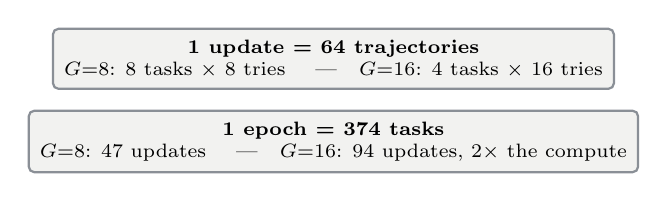
\begin{tikzpicture}[font=\scriptsize]
  \node[boxg, minimum width=4.6cm] (step) at (0,0) {\textbf{1 update = 64 trajectories}\\ $G{=}8$: 8 tasks $\times$ 8 tries \quad|\quad $G{=}16$: 4 tasks $\times$ 16 tries};
  \node[boxg, minimum width=4.6cm, below=0.25cm of step] (ep) {\textbf{1 epoch = 374 tasks}\\ $G{=}8$: 47 updates \quad|\quad $G{=}16$: 94 updates, 2$\times$ the compute};
\end{tikzpicture}
\end{center}
\column{0.48\textwidth}
\scriptsize
\begin{tabular}{@{}llc@{}}
\toprule
\textbf{Name} & \textbf{Content} & $G$ \\
\midrule
\rowcolor{crGrey}\multicolumn{3}{@{}l}{\textbf{References}} \\
\textsc{Replication-FT} & paper recipe, full finetuning, fixed reference & 8 \\
\textsc{Moving-Anchor} & ReLoRA $r{=}8$: adapter merged and restarted, KL reference moved every 4 epochs & 8 \\
\rowcolor{crGrey}\multicolumn{3}{@{}l}{\textbf{Controls}} \\
\textsc{Control-G16} & \textsc{Moving-Anchor} recipe, no curriculum & 16 \\
\textsc{Control-G16 + bound} & same, per-token KL bounded at 10 (verl) & 16 \\
\rowcolor{crGrey}\multicolumn{3}{@{}l}{\textbf{Curricula (\textsc{Moving-Anchor} recipe)}} \\
\textsc{Horizon} & interaction turns increasing by stages & 16 \\
\textsc{Budget} & tokens per turn increasing by stages & 16 \\
\textsc{Depth} & recipe depth increasing & 16 \\
\bottomrule
\end{tabular}
\end{columns}
\end{frame}

\begin{frame}{Preconditions: mask observations, keep the reward binary}
\begin{columns}[T]
\column{0.5\textwidth}
\textbf{Mask observations without removing them}
\begin{center}
\resizebox{\textwidth}{!}{%
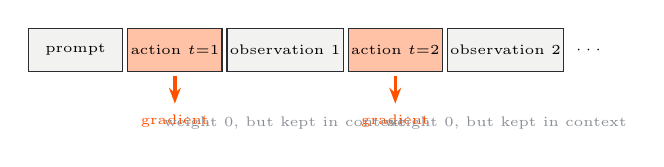
\begin{tikzpicture}[font=\tiny]
  \node[tok, fill=crGrey, minimum width=1.2cm] (p) at (0,0) {prompt};
  \node[tok, fill=crOrange!35, minimum width=1.0cm, right=0.05cm of p] (a1) {action $t{=}1$};
  \node[tok, fill=crGrey, minimum width=1.2cm, right=0.05cm of a1] (o1) {observation 1};
  \node[tok, fill=crOrange!35, minimum width=1.0cm, right=0.05cm of o1] (a2) {action $t{=}2$};
  \node[tok, fill=crGrey, minimum width=1.2cm, right=0.05cm of a2] (o2) {observation 2};
  \node[tok, draw=none, right=0.05cm of o2] (dots) {$\cdots$};
  \draw[arro] ($(a1.south)+(0,-0.05)$) -- ++(0,-0.35) node[below, text=crOrange] {gradient};
  \draw[arro] ($(a2.south)+(0,-0.05)$) -- ++(0,-0.35) node[below, text=crOrange] {gradient};
  \node[below=0.45cm of o1, text=crMid] {weight 0, but kept in context};
  \node[below=0.45cm of o2, text=crMid] {weight 0, but kept in context};
\end{tikzpicture}}
\end{center}
\footnotesize
\begin{itemize}
  \item Observation tokens get zero weight in the loss, but stay in the sequence.
  \item Remove them and every action is scored out of context.
  \item Silent failure: the loss decreases, the model learns nothing.
\end{itemize}
\column{0.5\textwidth}
\textbf{A warning against reward shaping}
\footnotesize
\begin{itemize}
  \item Tried: $+0.02$ for exactly one action, $-0.05$ otherwise, $-0.01$ per invalid action. Three magic numbers.
  \item In a group with no success, this term is the \emph{only} one that varies.
  \item Twenty updates later: outputs under 100 tokens, reward $>1$, zero tasks solved. The policy learned to \emph{give up cleanly}.
  \item GRPO's division by the standard deviation makes it worse: a $0.02$ gap becomes a full-size advantage (Dr.~GRPO).
  \item Binary reward kept, as in DeepSeek-R1.
\end{itemize}
\end{columns}
\refs{DeepSeek-R1 2025 ; Liu et al. 2025 (Dr.~GRPO) ; Skalse et al. 2022}
\end{frame}

\begin{frame}{Full-finetuning replication}
\begin{columns}[T]
\column{0.58\textwidth}
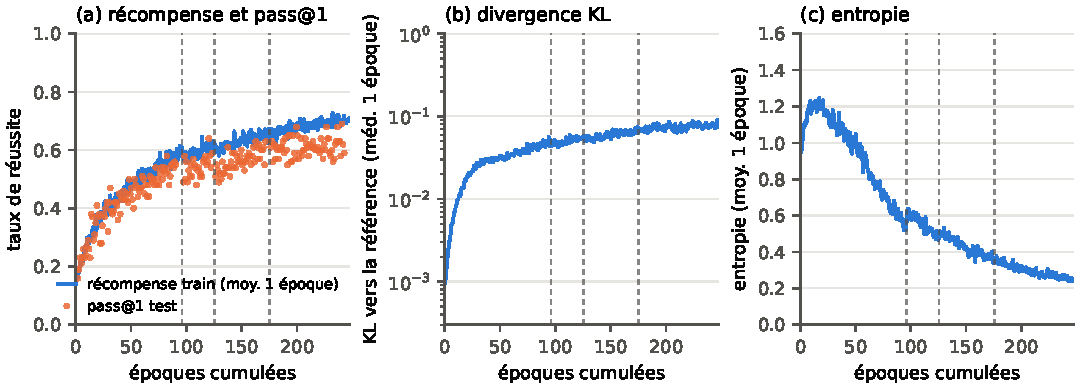
\includegraphics[width=\textwidth]{fig_fullft_stabilite.pdf}
\vspace{0.15cm}
\begin{keymsg}
The reference exists. It is too slow and too costly to build on. We need a way to efficiency.
\end{keymsg}
\column{0.4\textwidth}
\small
\begin{itemize}
  \item Same hyperparameters as the paper's code.
  \item Ported to a single GPU; the training engine rewritten from verl to TRL.
  \item 40\% at epoch 30, where the paper reports 75. \hl{69\%} after 247 epochs, plateau 61.
  \item No collapse: KL slow and linear, entropy sharpening.
  \item \hl{Over 200 GPU hours}, 12 GB per checkpoint. No co-located inference engine at the time, all weights in the optimizer.
\end{itemize}
\end{columns}
\end{frame}

% ---- LoRA
\begin{frame}{Efficiency: from the paper to our adapter}
\begin{columns}[T]
\column{0.5\textwidth}
\textbf{What made the rest possible}
\begin{itemize}
  \item Machine migration (new glibc): recent TRL + co-located vLLM, generation and training in one process. Updates three times faster.
  \item Start from the paper's full-finetuning recipe, train only an adapter.
  \item Our adapter: rank 8, $\alpha=32$, on all linear layers.
  \item Hyperparameters re-tuned by a grid: learning rate $3\cdot10^{-6}$ instead of $10^{-6}$, $\beta=10^{-2}$ instead of $10^{-3}$.
\end{itemize}
\column{0.5\textwidth}
\textbf{What it changes}
\begin{itemize}
  \item 180 MB per checkpoint instead of 12 GB.
  \item The freed memory will allow $G=16$ and hyperparameter grids.
  \item Natural KL reference: the base model, adapter disabled.
\end{itemize}
\vspace{0.2cm}
\begin{center}\kpi{100}{$\times$ less optimizer memory}\end{center}
\end{columns}
\refs{Hu et al. 2022 (LoRA) ; Schulman et al. 2025 (LoRA Without Regret)}
\end{frame}

\begin{frame}{LoRA with a fixed reference: exponential KL drift}
\begin{columns}[T]
\column{0.6\textwidth}
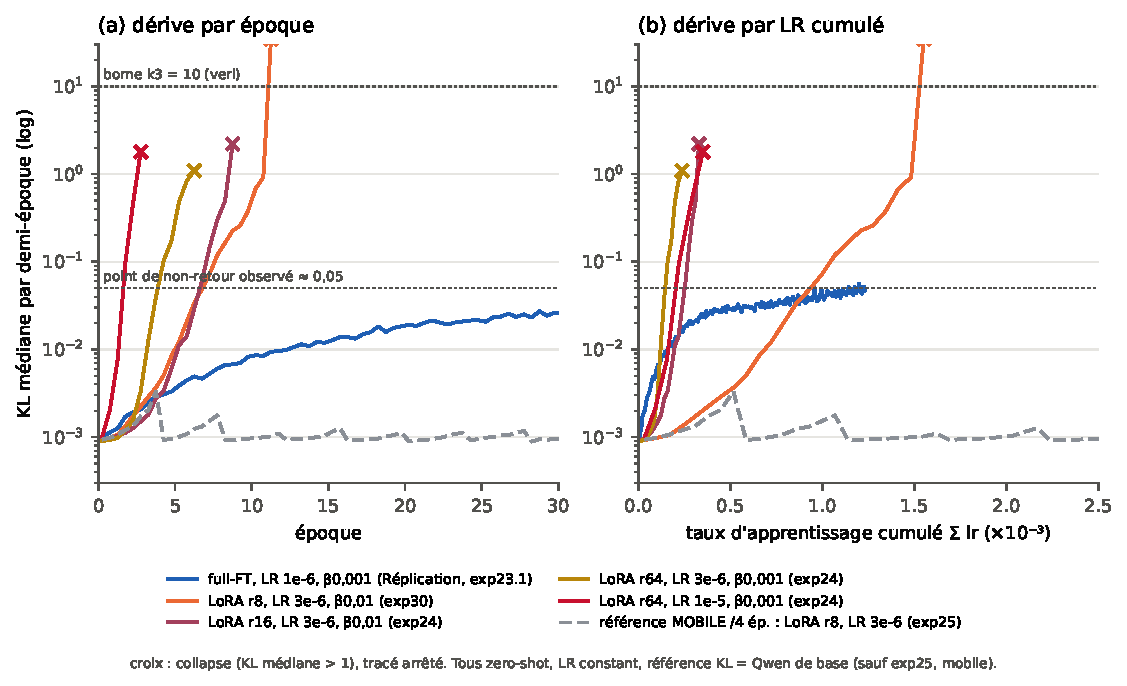
\includegraphics[width=\textwidth]{fig_kl_drift_fixed_anchor.pdf}
\column{0.38\textwidth}
\small
\begin{itemize}
  \item Fixed reference = the base model, as in the paper.
  \item Every LoRA of the grid collapsed between epochs 3 and 11. Only full finetuning holds.
  \item Full finetuning: \hl{linear} drift, $+0.0015$ per two epochs.
  \item LoRA: \hl{exponential} drift, $\times 5$ to $\times 20$ per two epochs, whatever the rank or $\beta$.
  \item The learning rate sets the speed, not the shape (panel b).
\end{itemize}
\end{columns}
\vspace{0.1cm}
\begin{keymsg}
Why the KL brake comes too late: in a healthy regime $\beta\cdot$KL is $10^{-5}$ against $3\cdot10^{-3}$ for the policy term. It only engages at KL $\approx 0.3$. Fine against a linear drift, too late against an exponential one. Hypothesis: the LoRA delta is a product $B\cdot A$ whose two factors grow, so drift speed grows with the distance already travelled.
\end{keymsg}
\end{frame}

\begin{frame}{Fix: a moving KL reference by merge-and-restart. This is ReLoRA}
\begin{columns}[T]
\column{0.56\textwidth}
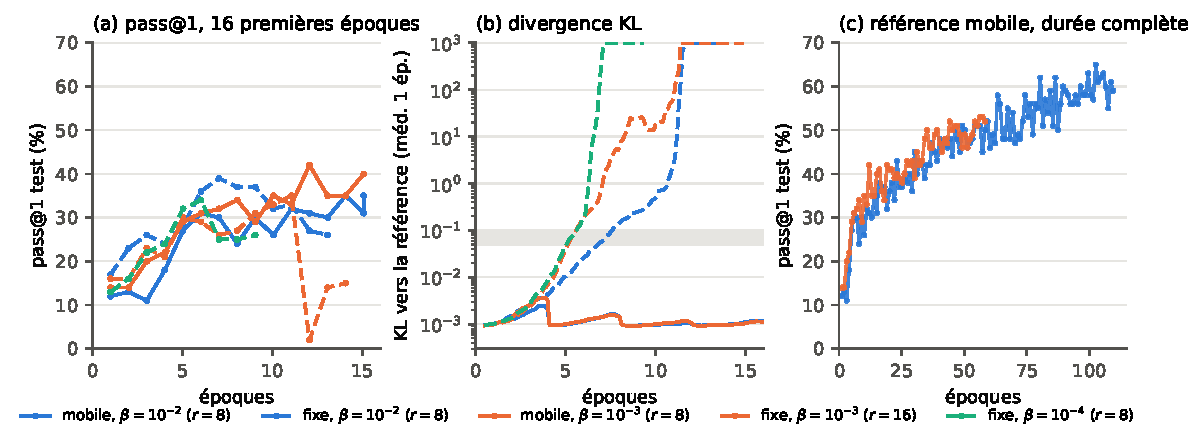
\includegraphics[width=\textwidth]{fig_anchor_square.pdf}
\column{0.42\textwidth}
\small
\begin{itemize}
  \item We need a reference that follows the policy.
  \item TRL can do it for a full model, not with an adapter: its reference is the base without adapter, by construction.
  \item Least invasive workaround, every four epochs: \hl{merge} the adapter into the base, \hl{restart} it at zero, purge the optimizer.
  \item Result: KL at $10^{-3}$ for 111 epochs. 65, then \hl{73\%}, at LoRA cost.
  \item Fixed vs. moving $\times$ $\beta$: the reference regime governs, not $\beta$.
  \item This has a name, found afterwards: \textbf{ReLoRA}. The accumulated delta is a sum of rank-8 deltas, rank 160 after twenty cycles.
\end{itemize}
\end{columns}
\vspace{0.05cm}
\begin{keymsg}
Not a mathematical constraint: a TRL/PEFT implementation limit, plus our choice of the least invasive workaround. A no-reset alternative, a frozen copy of the adapter as reference, remains to be tested.
\end{keymsg}
\refs{Lialin et al. 2023 (ReLoRA) ; Liu et al. 2025 (ProRL) ; Schulman et al. 2015 (TRPO)}
\end{frame}

\begin{frame}{What the adaptation bought: compute per lineage}
\begin{columns}[T]
\column{0.58\textwidth}
\small\setlength{\tabcolsep}{4pt}
\begin{tabular}{@{}lrrrrr@{}}
\toprule
 & updates & GPU h & tokens & env. turns & plateau \\
\midrule
\textsc{Replication-FT} & 11\,564 & 238 & 0.87 G & 12.4 M & 61 \\
\textsc{Moving-Anchor} $G{=}8$ & 8\,018 & 70 & 0.62 G & 8.6 M & 70 \\
\textsc{Horizon} & 7\,518 & 48 & 0.45 G & 6.3 M & 78 \\
\textsc{Budget} & 7\,194 & 51 & 0.43 G & 7.2 M & 75 \\
\textsc{Depth} & 7\,904 & 66 & 0.56 G & 7.9 M & 74 \\
\textsc{Control-G16} & 1\,434 & 16 & 0.15 G & 1.9 M & collapse \\
\bottomrule
\end{tabular}
\vspace{0.15cm}
{\scriptsize Environment turns estimated from the mean number of turns per depth and per stage.}
\column{0.4\textwidth}
\begin{itemize}
  \item Replication: 238 hours for 61. ReLoRA: 70 hours for 70.
  \item \hl{Three times less time, nine more points}, 180 MB per checkpoint instead of 12 GB.
  \item Curricula of means cut the episodes: cheaper per update still.
  \item This gain made the grids, controls and curricula possible.
\end{itemize}
\end{columns}
\end{frame}

\begin{frame}{Stabilization at $G=8$: fixed vs. moving reference}
\begin{columns}[T]
\column{0.62\textwidth}
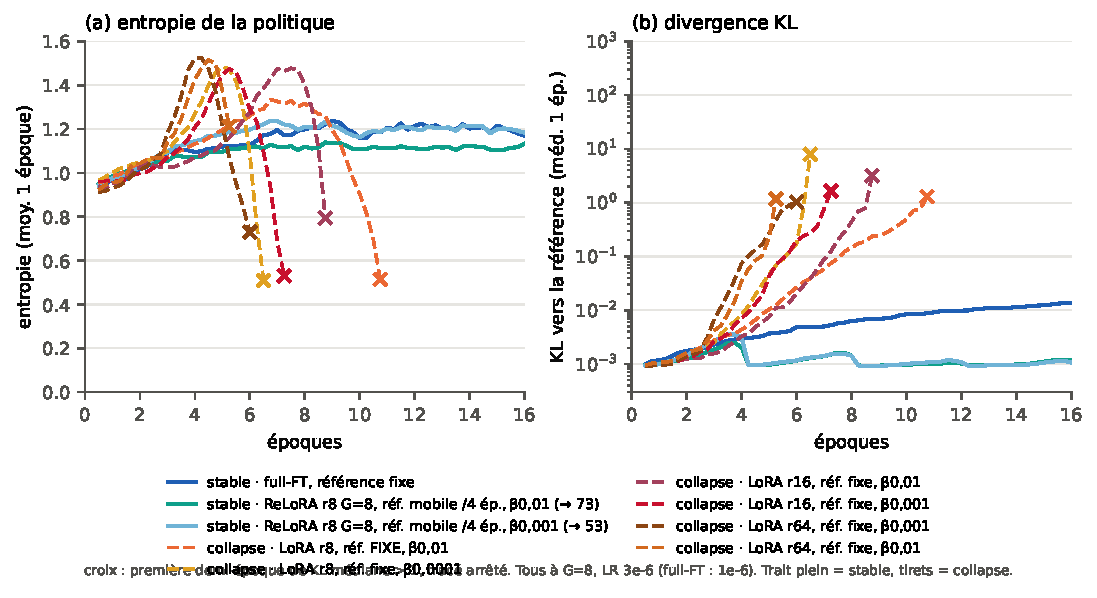
\includegraphics[width=\textwidth]{fig_collapse_signals_a.pdf}
\column{0.36\textwidth}
\footnotesize
Nine runs at $G=8$, first sixteen epochs. Solid: stable. Dashed: collapse, stopped at the cross.
\begin{itemize}
  \item \textbf{Fixed reference, LoRA}: KL exponential from epoch 3, entropy \emph{rises} then falls. \hl{KL first.} No rank, no $\beta$ saves it.
  \item \textbf{Fixed reference, full finetuning}: linear KL, constant entropy, stable.
  \item \textbf{Moving reference}: KL reset to $10^{-3}$ every cycle, entropy stable at 1.1, at two $\beta$.
\end{itemize}
\vspace{0.1cm}
\begin{keymsg}
At $G=8$, LoRA with a moving reference reaches \hl{73\%} and does not collapse. Can we do better with it?
\end{keymsg}
\end{columns}
\end{frame}

\begin{frame}{Going to $G=16$: a better gradient, and a new collapse}
\begin{columns}[T]
\column{0.62\textwidth}
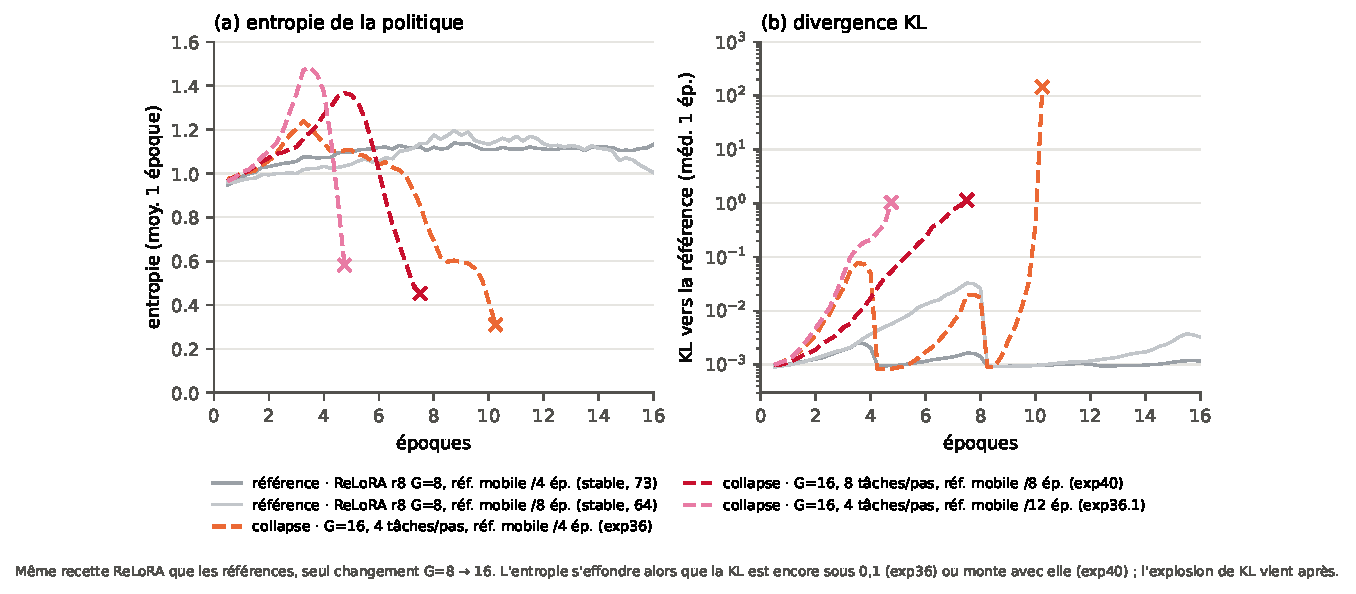
\includegraphics[width=\textwidth]{fig_collapse_signals_b.pdf}
\column{0.36\textwidth}
\footnotesize
\textbf{Why $G=16$.} LoRA freed the memory. Twice as many tries per task: a better advantage estimate, and twice the chance that a hard task is mixed.
\vspace{0.1cm}

\textbf{What happens.} Same recipe, only $G=8\to16$. The control rises faster (54 at epoch 8) and dies at epoch 10. Two variants, slower anchor or eight tasks per step: same end.
\vspace{0.1cm}
\begin{keymsg}
\hl{Entropy first.} It collapses while KL is still below 0.1; the KL explosion comes after. A second collapse mode the moving reference does not see. H1 confirmed.
\end{keymsg}
\end{columns}
\end{frame}

\begin{frame}{Proposed mechanism: mixed groups, entropy, shrinking turns}
\begin{columns}[T]
\column{0.5\textwidth}
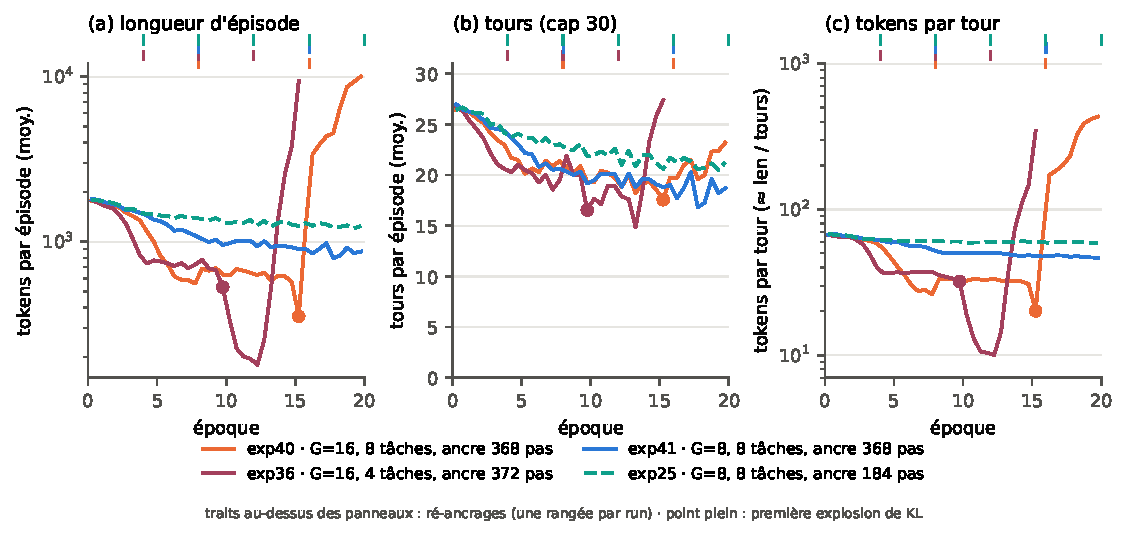
\includegraphics[width=\textwidth]{fig_collapse_lengths.pdf}
\column{0.48\textwidth}
\footnotesize
\begin{itemize}
  \item Only mixed groups give gradient. Without curriculum, hard tasks are mixed from the start, more so at $G=16$.
  \item In such a group: one short routine success (\hl{exploitation}, reinforced) against fifteen long failures full of rare actions (\hl{exploration}, punished token by token).
  \item Cui et al. 2025: entropy falls, nothing recharges it. At the floor, the policy freezes.
  \item Measured: at $G=16$ turns shrink from 65 to 30 tokens by epoch 5. The ``Thought'' disappears. At $G=8$ they stay at 45-60.
  \item The number of turns does not change. Each turn empties out.
\end{itemize}
\vspace{0.05cm}
\begin{keymsg}
Measured: entropy, turn length, KL. Not measured: the share of mixed groups, the covariance of Cui et al. A consistent hypothesis, not a proof.
\end{keymsg}
\end{columns}
\refs{Cui et al. 2025 (The Entropy Mechanism of RL for Reasoning LMs)}
\end{frame}

\begin{frame}{What a curriculum can bring here}
\begin{itemize}\setlength{\itemsep}{4pt}
  \item A curriculum decides \emph{when} a task may produce gradient.
  \item Tasks out of reach do not punish yet. Failures are short. Next-stage successes come from rare actions. It \hl{recharges exploration}.
  \item At $G=16$, this is exactly what is missing: mixed groups arrive too early, on the wrong tasks.
  \item Three ways to do it, identical recipe: ration the horizon, ration the token budget, order recipes by depth.
  \item No curriculum at $G=8$ in this campaign (decision of August 24, speed and homogeneity). The missing run is in progress.
\end{itemize}
\vspace{0.3cm}
\begin{keymsg}
H3 in two parts: a curriculum \emph{protects} from the entropy collapse, and it \emph{accelerates}. The next runs test the first. The second needs an equal-compute comparison, done further on.
\end{keymsg}
\end{frame}

\begin{frame}{Three curriculum regimes, one common recipe}
Common recipe: ReLoRA $r{=}8$, learning rate $3\cdot10^{-6}$, $\beta=10^{-2}$, moving reference every four epochs, $G=16$, 80 epochs.
\vspace{0.2cm}
\begin{columns}[T]
\column{0.32\textwidth}
\begin{block}{Horizon}
Interaction turns: 10, then 20, then 30. ScalingInter revisited.
\end{block}
\column{0.32\textwidth}
\begin{block}{Budget}
Tokens per turn: 256, then 512, then 1024. Same family, another harness parameter.
\end{block}
\column{0.32\textwidth}
\begin{block}{Depth}
Recipes of depth $\le 1$, then $\le 2$, $\le 3$, $\le 4$. Next stage when training reward exceeds 0.8.
\end{block}
\end{columns}
\vspace{0.3cm}
\begin{itemize}
  \item Two levers: \hl{ration the means} (Horizon, Budget) or \hl{order the tasks} (Depth).
  \item Two references without curriculum: \textsc{Moving-Anchor} at $G=8$ (73\%) and \textsc{Control-G16}, same recipe as the curricula.
\end{itemize}
\end{frame}

\begin{frame}{Schedules of the three curricula}
\begin{center}
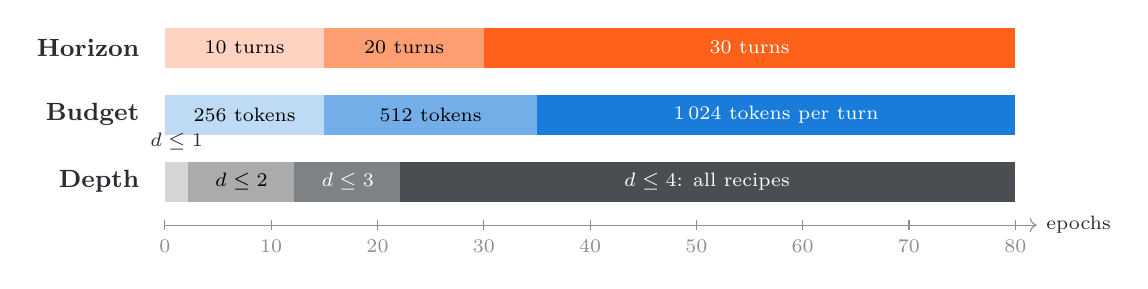
\begin{tikzpicture}[x=0.135cm,y=0.85cm,font=\scriptsize]
  % epoch axis
  \draw[crMid,->] (0,-0.35) -- (82,-0.35) node[right,crDark] {epochs};
  \foreach \e in {0,10,20,30,40,50,60,70,80} {\draw[crMid] (\e,-0.28) -- (\e,-0.42) node[below,crMid] {\e};}
  % Horizon
  \node[anchor=east,crDark,font=\small\bfseries] at (-1.5,2.3) {Horizon};
  \fill[crOrange!25] (0,2) rectangle (15,2.6);  \node at (7.5,2.3) {10 turns};
  \fill[crOrange!55] (15,2) rectangle (30,2.6); \node at (22.5,2.3) {20 turns};
  \fill[crOrange!90] (30,2) rectangle (80,2.6); \node[white] at (55,2.3) {30 turns};
  % Budget
  \node[anchor=east,crDark,font=\small\bfseries] at (-1.5,1.3) {Budget};
  \fill[crBlue!25] (0,1) rectangle (15,1.6);  \node at (7.5,1.3) {256 tokens};
  \fill[crBlue!55] (15,1) rectangle (35,1.6); \node at (25,1.3) {512 tokens};
  \fill[crBlue!90] (35,1) rectangle (80,1.6); \node[white] at (57.5,1.3) {1\,024 tokens per turn};
  % Depth (adaptive stages, observed epochs)
  \node[anchor=east,crDark,font=\small\bfseries] at (-1.5,0.3) {Depth};
  \fill[crDark!20] (0,0) rectangle (2.14,0.6);
  \fill[crDark!40] (2.14,0) rectangle (12.14,0.6); \node at (7.2,0.3) {$d\le2$};
  \fill[crDark!60] (12.14,0) rectangle (22.14,0.6); \node[white] at (17.2,0.3) {$d\le3$};
  \fill[crDark!85] (22.14,0) rectangle (80,0.6); \node[white] at (51,0.3) {$d\le4$: all recipes};
  \node[anchor=south,crDark] at (1.1,0.62) {$d\le1$};
\end{tikzpicture}
\end{center}
\footnotesize
\begin{itemize}\setlength{\itemsep}{1pt}
  \item \textsc{Horizon}, \textsc{Budget}: long fixed stages, so each level can saturate. The paper switches every 100 updates, about two epochs.
  \item \textsc{Depth}: next stage once training reward exceeds 0.8 over an epoch, or after 10 epochs. Observed: 2.1, 12.1, 22.1.
  \item The fixed-schedule version (0, 12, 25, 37) saturated: six epochs without gradient at stage 1.
  \item A stage changes: the truncated episode (Horizon), the truncated answer (Budget), the sampled tasks (Depth).
\end{itemize}
\end{frame}

\begin{frame}{Curriculum results: pass@1 and entropy}
\begin{columns}[T]
\column{0.58\textwidth}
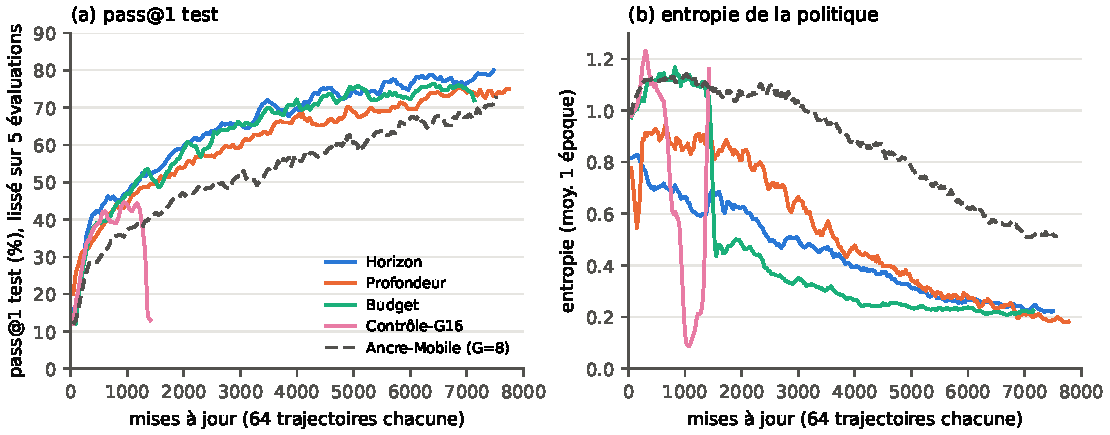
\includegraphics[width=\textwidth]{fig_curricula_pass1_entropy.pdf}
\column{0.4\textwidth}
\footnotesize\setlength{\tabcolsep}{4pt}
\begin{tabular}{@{}lrr@{}}
\toprule
 & plateau & best \\
\midrule
\textsc{Horizon} & \textbf{78} & \textbf{82} \\
\textsc{Budget} & 75 & 80 \\
\textsc{Depth} & 74 & 80 \\
\textsc{Moving-Anchor} $G{=}8$ & 70 & 73 \\
\textsc{Replication-FT} & 61 & 69 \\
\textsc{Control-G16} & \multicolumn{2}{c}{54 then collapse} \\
\bottomrule
\end{tabular}
\vspace{0.2cm}
\begin{itemize}\setlength{\itemsep}{2pt}
  \item The control dies at epoch 10. The three curricula hold 80 epochs. Protection acquired.
  \item Their entropy goes lower than the $G=8$ reference, but over 60 epochs with a rising pass@1. Sharpening, not collapse.
  \item Paper: 75. All three exceed it.
\end{itemize}
\end{columns}
\end{frame}

\begin{frame}{Results by depth and by error class}
\begin{columns}[T]
\column{0.5\textwidth}
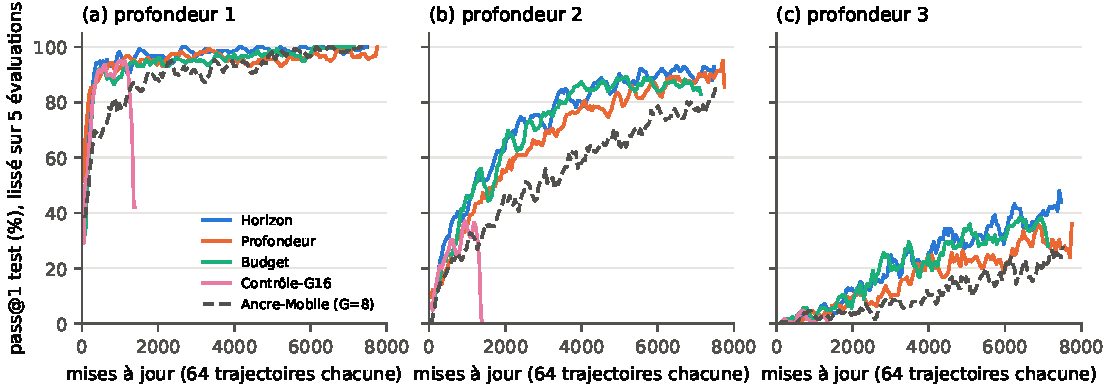
\includegraphics[width=\textwidth]{fig_curricula_depths.pdf}
\column{0.5\textwidth}
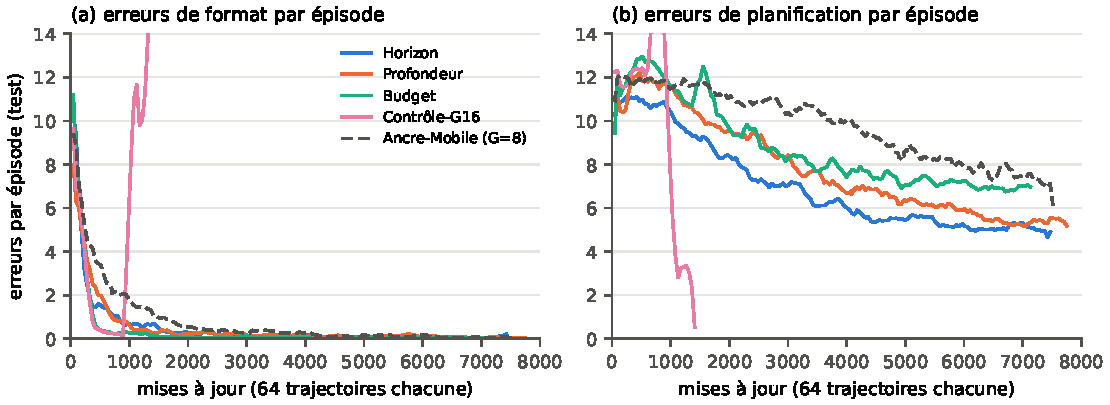
\includegraphics[width=\textwidth]{fig_curricula_errors.pdf}
\end{columns}
\vspace{0.2cm}
\begin{itemize}
  \item Depth 1 learned in five epochs. Depth 2 near 90\%. Depth 3 between 30 and 45\%. Depth 4 never.
  \item The oracle's capacity wall moved for depth 3 (0 in 500 draws before training), not for depth 4.
  \item A model trained to 32\% already solves at 20 tries 14 depth-2 and 2 depth-3 tasks the base never solved (pass@20 65). \textsc{Horizon} makes 82 in one try, above the base's pass@20 (47).
  \item ProRL rather than Yue et al., up to a point: $k=20$ is small.
  \item Curricula accelerate without changing the order of acquisition. Format errors gone in under a thousand updates. Planning errors slow.
\end{itemize}
\end{frame}

\begin{frame}{A naive method against the curricula: bound the KL in the loss}
\begin{columns}[T]
\column{0.58\textwidth}
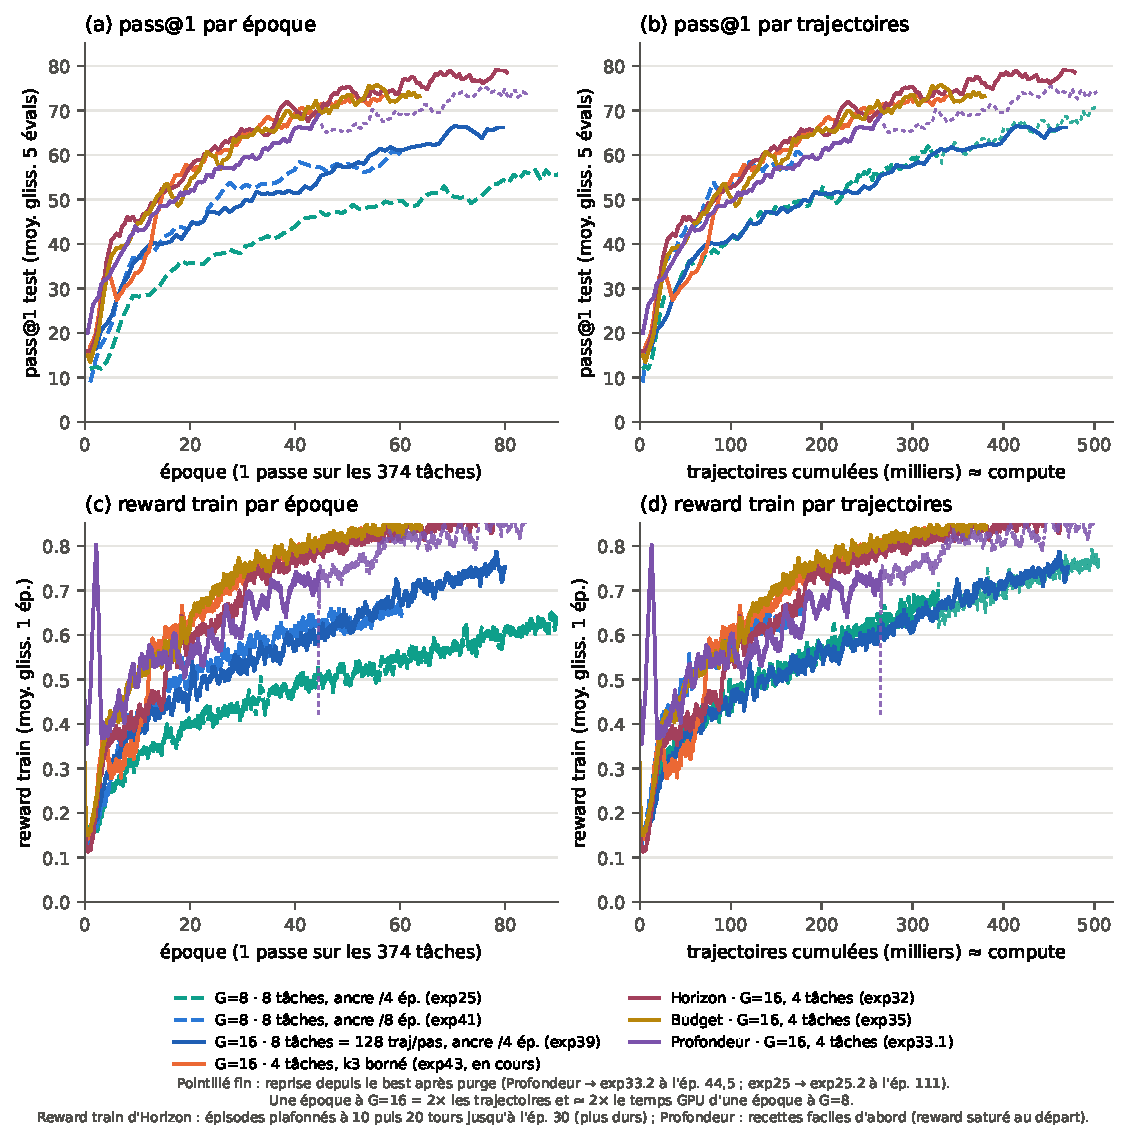
\includegraphics[width=\textwidth]{fig_g8_vs_g16_curricula.pdf}
\column{0.4\textwidth}
\footnotesize
\textbf{Where the KL explosion comes from.} Token-by-token replay of the control. The $k_3$ estimator is unbounded in TRL, bounded at 10 in the paper's stack. Once the policy is peaked, a token it eliminated but the reference expects weighs $10^{7}$ to $10^{19}$ in the loss. KL is not the cause. It is the thermometer that breaks.
\vspace{0.1cm}

\textbf{The test.} Control $G=16$ + bound at 10, one delta. In progress, epoch 22. It passes epochs 10 and 15, where the controls died. KL bounded, no loops. But entropy collapses \emph{earlier} (0.11 at epoch 4): the bound removes the brake on the tokens that drift, nothing holds the sharpening.
\vspace{0.1cm}
\begin{keymsg}
At equal compute, bound and curricula are indistinguishable up to 120k trajectories (55-58). Then curricula go to 70-80 at entropy 0.6; the bound runs at 0.33. Divergence avoided, exploration not. Verdict at the plateau.
\end{keymsg}
\end{columns}
\end{frame}

\begin{frame}{$G=8$ vs. $G=16$ at equal compute}
\begin{columns}[T]
\column{0.58\textwidth}
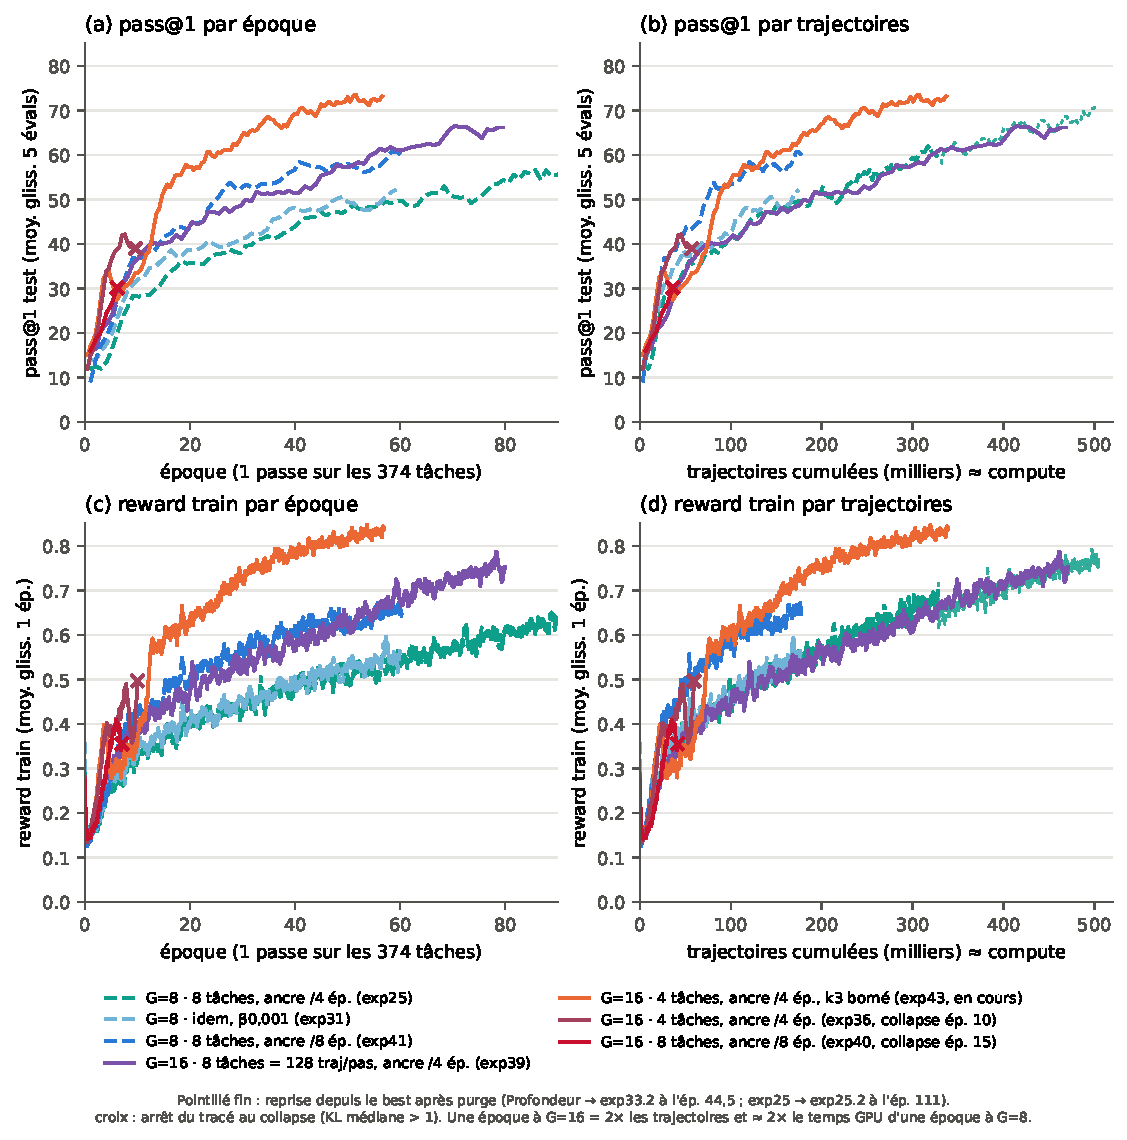
\includegraphics[width=\textwidth]{fig_g8_vs_g16.pdf}
\column{0.4\textwidth}
\footnotesize
\begin{itemize}
  \item One epoch at $G=16$ is twice the trajectories and GPU time of one at $G=8$. The right column compares at equal compute.
  \item Only delta $G$ (same 8 tasks per step): at 180k trajectories, $G=8$ is at 60, $G=16$ at 50. \hl{Nothing shows that $G$ accelerates.}
  \item Surprise: two $G=8$ runs identical except the re-anchoring period, 4 or 8 epochs: 49 vs. 60. Each merge-and-restart purges Adam. The cost shows.
  \item Curricula stay above every no-curriculum run beyond 200k trajectories.
\end{itemize}
\vspace{0.1cm}
\begin{keymsg}
H3: the curriculum protects (established) and raises the plateau (established at equal compute). Early acceleration not shown. The clean $G=8$ comparison is running.
\end{keymsg}
\end{columns}
\end{frame}

% =====================================================================
\section{Conclusion and outlook}

\begin{frame}{Contributions}
\begin{enumerate}
  \item \textbf{A scoping.} From an open topic on self-improvement to a precise question: the difficulties of RL training for a multi-turn agent, and the conditions for stability and efficiency. A literature synthesis organized as testable hypotheses.
  \item \textbf{A replication at equal conditions} on one GPU: 69\% in full finetuning. And an efficient recipe that holds: \hl{73\%} with ReLoRA and a moving reference, at a third of the cost.
  \item \textbf{Three training regimes characterized} on sixteen runs: full finetuning with fixed reference (stable, linear); LoRA with fixed reference (exponential drift, KL collapse); ReLoRA with moving reference (stable at $G=8$, entropy collapse at $G=16$). The KL explosion mechanism identified token by token.
  \item \textbf{Curriculum as protection and as a higher plateau}, identical recipe, controlled compute: three regimes that hold where the control breaks, up to \hl{82\%} for 75 in the paper.
\end{enumerate}
\vspace{0.15cm}
\begin{keymsg}
And a reproducible infrastructure: training, evaluation, token-level replay, logs and recipes, ready for another environment.
\end{keymsg}
\end{frame}

\begin{frame}{Scope of validity and perspectives}
\footnotesize
\begin{columns}[T]
\column{0.48\textwidth}
\textbf{What the results allow}
\begin{itemize}
  \item \emph{Internal} comparisons, identical recipe, measured compute.
  \item Stability conditions independent of the model: masking, binary reward, reference regime, bounded KL estimator, difficulty rationing.
\end{itemize}
\textbf{What they do not allow}
\begin{itemize}
  \item One run per configuration. One environment, one 3B model, one GPU.
  \item The gap with the paper at equal budget remains unexplained.
  \item $G$ and re-anchoring period are now separated. Accumulated capacity and moving reference are not yet.
\end{itemize}
\column{0.5\textwidth}
\textbf{What they call for}
\begin{itemize}
  \item Rebalance the training set by depth, then rerun the chain in order: LoRA fixed reference, moving reference, curriculum.
  \item Repeat the decisive runs with several seeds.
  \item Test the recipe on the other AgentGym-RL environments, then on Criteo's shopping environment, where the reward is neither binary nor exact.
\end{itemize}
\textbf{What they open}
\begin{itemize}
  \item Combine the curriculum levers; their effects need not add up.
  \item Autotelic agents: let the model order its own tasks, on a stabilized base.
\end{itemize}
\end{columns}
\end{frame}

\begin{frame}{Value for Criteo}
\begin{columns}[T]
\column{0.5\textwidth}
\textbf{What Criteo gets}
\begin{itemize}
  \item A structured synthesis of RL training for agents, as hypotheses and failure conditions.
  \item A reusable technical brick: TRL + co-located vLLM on one GPU, LoRA/ReLoRA with moving reference, KL bound, curricula, evaluation and token-level replay.
  \item The conditions for training that works, independent of the model. They are what matters on a proprietary environment no model has seen.
\end{itemize}
\column{0.5\textwidth}
\begin{block}{Kein's work}
\small \textit{[To complete: short presentation of Kein's work and how it connects to this internship.]}
\end{block}
\vspace{0.2cm}
\begin{keymsg}
What does not depend on us: Qwen3.5-4B without training makes 78.5\% on TextCraft, one year after Qwen2.5. What depends on us: knowing how to train on an environment nobody has seen.
\end{keymsg}
\end{columns}
\end{frame}

\begin{frame}{The last month: running, and next}
\small
\begin{columns}[T]
\column{0.5\textwidth}
\textbf{Running and queued}
\begin{itemize}
  \item \textsc{Control-G16 + bound}: to the plateau. Is the bound enough?
  \item \textsc{Horizon} at $G=8$: the curriculum isolated from $G$, against \textsc{Moving-Anchor} and \textsc{Horizon} $G=16$.
  \item Resume of the $G=8$ slow-anchor reference to 80 epochs.
\end{itemize}
\column{0.5\textwidth}
\textbf{Next, by increasing cost}
\begin{itemize}
  \item True LoRA $r=8$ with a moving reference, no merge, no reset: separates moving reference from accumulated capacity. Then $r=64$ if it plateaus.
  \item LoRA with fixed reference + KL bound: does the bound replace the anchor?
  \item LoRA with fixed reference at the full-finetuning learning rate: close the learning-rate question.
  \item Rebalance the dataset by depth, repeat the decisive runs.
\end{itemize}
\end{columns}
\vspace{0.2cm}
\begin{keymsg}
Every one of these is a single delta to the stabilized recipe. That is what the campaign made possible.
\end{keymsg}
\end{frame}

\begin{frame}{Outlook: autocurriculum and autotelic agents}
\begin{columns}[T]
\column{0.5\textwidth}
\textbf{From fixed to measured difficulty}
\begin{itemize}
  \item Our curricula fix the order by hand. An \textbf{autocurriculum} picks difficulty from a criterion measured on the learner (Portelas 2020), such as \emph{learning progress} (Graves 2017).
  \item \textbf{Autotelic agents} (Colas et al. 2022; Oudeyer and Kaplan 2007) set their own goals in a large space, driven by intrinsic motivation.
  \item \textbf{MAGELLAN} (Gaven et al. 2025): a competence head on the LLM's hidden state; progress $= |$prediction $-$ delayed prediction$|$; goals sampled proportionally to progress.
\end{itemize}
\column{0.5\textwidth}
\textbf{What we tried}
\begin{itemize}
  \item MAGELLAN ported to TextCraft. Prediction written before the run: it will give up on depth 4. Verified: $p(d_4)=0.0006$ at the end.
  \item 45\% at epoch 6, then collapse at epochs 7-8, earlier than the control.
  \item Progress measures change, and a collapse is a change. The estimator put 79\% of sampling on depth 1 and sped up the failure.
\end{itemize}
\begin{keymsg}
Requirement: a stable learner. Next step: plug the autocurriculum on the curriculum-stabilized recipe, where difficulty is not known in advance.
\end{keymsg}
\end{columns}
\refs{Portelas 2020 ; Graves 2017 ; Colas et al. 2022 ; Oudeyer and Kaplan 2007 ; Gaven et al. 2025 (MAGELLAN) ; report appendix E}
\end{frame}

{
\setbeamercolor{background canvas}{bg=crDark}
\setbeamertemplate{footline}{}
\begin{frame}[plain]
  \vfill
  \begin{center}
    {\color{crOrange}\rule{2.4cm}{3pt}}\\[0.6cm]
    {\color{white}\fontsize{26}{30}\selectfont\bfseries Thank you.\par}
    \vspace{0.4cm}
    {\color{white}\large Questions?\par}
    \vspace{1cm}
    {\color{crMid}\small Report, code, recipes and logs: repository \texttt{rl-gym-workout}}
  \end{center}
  \vfill
\end{frame}
}

% =====================================================================
\appendix
\inappendixtrue
\section{Appendix}

\begin{frame}{B1. SNIS: recombining trajectories within a group}
\begin{itemize}
  \item Idea: in a group, a thought $z_j$ and an answer $a_i$ from different trajectories form a valid pair. Reweight each pair by a self-normalized importance weight.
  \[ \tilde w_{ij} = \frac{\pi_\theta(a_i \mid x, z_j)}{\sum_{l} \pi_\theta(a_i \mid x, z_l)} \]
  \item Biased at finite $G$, consistent, reduced variance (Owen, ch. 9).
  \item In multi-turn, recombination breaks the causal link between observation and action. Collapse observed (exp17), stopped.
\end{itemize}
\refs{Report appendix B ; Owen 2013 ; Kazemnejad et al. 2024 (VinePPO)}
\end{frame}

\begin{frame}{B2. Single-turn planning vs. multi-turn control}
\begin{itemize}
  \item Qwen3.5-4B: 54\% with a full plan replayed, 77\% interactive. \hl{The feedback loop is worth 23 points.}
  \item Interactive RL policy: planning 12 $\to$ 19.5\% over eleven temperatures. Real but weak transfer: what RL learned is mostly reactive.
  \item Pure planning RL: 37\% in plan, 9\% interactive. It destroys the one-action-per-turn protocol.
  \item Not tested: alternating the two regimes.
\end{itemize}
\refs{Appendix D ; Dupoux, LeCun and Malik 2026}
\end{frame}

\begin{frame}{B3. Controls on $G$, tasks per step and re-anchoring period}
\begin{columns}[T]
\column{0.55\textwidth}
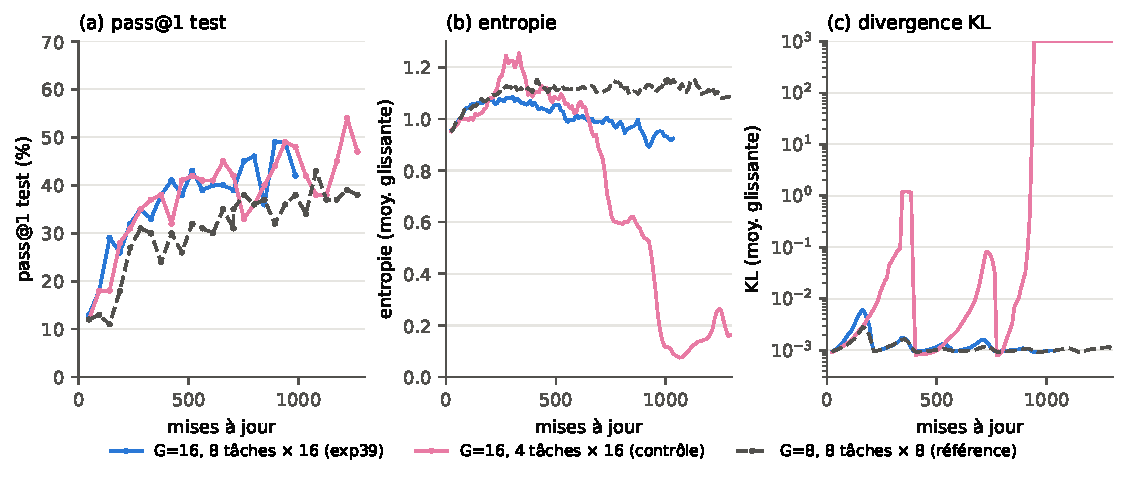
\includegraphics[width=\textwidth]{fig_exp39_control.pdf}
\column{0.43\textwidth}
\scriptsize\setlength{\tabcolsep}{3pt}
\begin{tabular}{@{}lccl@{}}
\toprule
Run & tasks $\times G$ & anchor (steps) & outcome \\
\midrule
\textsc{Moving-Anchor} & 8 $\times$ 8 & 184 & stable, 65 \\
exp41 & 8 $\times$ 8 & 368 & stable, 64 (ep. 60) \\
exp39 & 8 $\times$ 16 & 184 & stable, 72 (80 ep.) \\
exp40 & 8 $\times$ 16 & 368 & collapse ep. 15 \\
\textsc{Control-G16} & 4 $\times$ 16 & 372 & collapse ep. 10 \\
exp36.1 & 4 $\times$ 16 & 1116 & collapse ep. 5 \\
\textsc{Control-G16 + bound} & 4 $\times$ 16 & 372 & holds (ep. 22, best 63) \\
\bottomrule
\end{tabular}
\vspace{0.15cm}
\begin{itemize}
  \item At $G=8$, an anchor every 368 steps is enough. At $G=16$, only re-anchoring every 184 steps holds without curriculum or bound.
  \item Token-level replay (256 episodes per checkpoint): vLLM/HF gap median $10^{-5}$ nat, not the cause. At step 705 of the control: median turns of 12 tokens, 81\% without ``Thought''. After the explosion: 100\% of $k_3$ on the forced \texttt{<|im\_end|>} of looping truncated turns ($\rho=45$).
\end{itemize}
\end{columns}
\end{frame}

\begin{frame}{B4. KL divergence per run: reference, learning rate, $\beta$}
\scriptsize
\begin{tabular}{@{}lcccccl@{}}
\toprule
Run & reference & lr & $\beta$ & KL ep. 4-6 & KL ep. 8-10 & outcome \\
\midrule
Full-FT & fixed & $10^{-6}$ & $10^{-3}$ & 0.004 & 0.008 & stable, 0.08 at 247 ep. \\
LoRA r16 & fixed & $3\cdot10^{-6}$ & $10^{-3}$ & 0.040 & 17.7 & collapse ep. 8-10 \\
LoRA r16 & fixed & $3\cdot10^{-6}$ & $10^{-2}$ & 0.007 & 8.0 & collapse ep. 8-10 \\
LoRA r64 & fixed & $3\cdot10^{-6}$ & $10^{-3}$ & 0.83 (ep. 6) & — & collapse ep. 6 \\
LoRA r64 & fixed & $10^{-5}$ & $10^{-3}$ & 0.097 (ep. 2) & — & collapse ep. 3 \\
LoRA r8 & fixed & $3\cdot10^{-6}$ & $10^{-2}$ & 0.010 & 0.26 & collapse ep. 11 \\
LoRA r8 & fixed & $3\cdot10^{-6}$ & $10^{-4}$ & 0.047 & $10^{12}$ & divergence ep. 6-8 \\
ReLoRA r8 & moving & $3\cdot10^{-6}$ & $10^{-2}$ & 0.001 & 0.001 & stable 111 ep., 73 \\
ReLoRA r8 & moving & $3\cdot10^{-6}$ & $10^{-3}$ & 0.001 & 0.001 & stable 60 ep., 53 \\
\bottomrule
\end{tabular}
\vspace{0.3cm}
\small
\begin{itemize}
  \item The learning rate sets the drift speed (r64: $\times 80$ on KL at epoch 2 for $3\cdot10^{-6}\to10^{-5}$), the rank too. The exponential shape is LoRA's.
  \item Missing: a zero-shot LoRA at $10^{-6}$, the full-finetuning rate.
  \item $\beta=10^{-2}$ and $10^{-3}$ indistinguishable with a moving reference: 48.9 vs. 49.7 at epochs 49-58.
\end{itemize}
\end{frame}

\begin{frame}{B5. KL spikes: the $k_3$ estimator is unbounded in TRL}
\begin{columns}[T]
\column{0.6\textwidth}
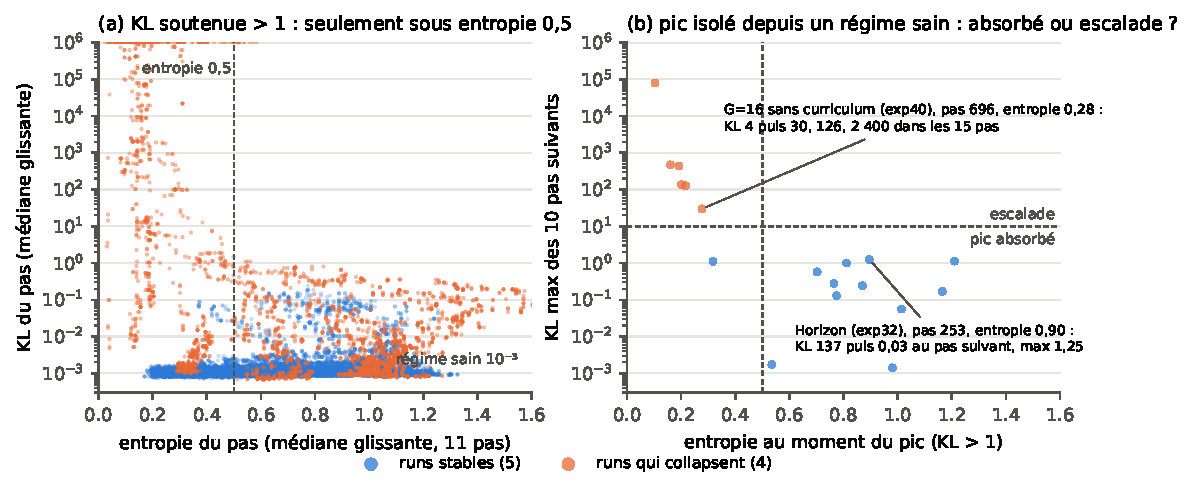
\includegraphics[width=\textwidth]{fig_collapse_entropy_kl.pdf}
\column{0.38\textwidth}
\small
\begin{itemize}
  \item Logged KL $= \overline{k_3}$ over sampled tokens, $k_3 = e^{\rho}-\rho-1$, $\rho = \log\pi_{\mathrm{ref}} - \log\pi$. verl bounds $k_3$ at 10 per token; \hl{TRL does not}.
  \item (a) Nine runs: a sustained KL $> 1$ only appears below entropy 0.5. Necessary, not sufficient (\textsc{Horizon} lives 20 epochs at 0.25).
  \item (b) Eighteen isolated spikes: 12 at entropy $> 0.5$, all absorbed; 6 at entropy $< 0.3$, all escalating.
  \item At step 705 of the control, the largest $k_3$ (300) are ``Thought'' tokens sampled at $p = 0.3\%$ where the reference gives 0.6: $\rho \approx 5$. After the explosion: $\rho = 45$, $k_3 = 10^{19}$ on forced end-of-turn tokens.
\end{itemize}
\end{columns}
\end{frame}

\begin{frame}{B6. Gap with the published results}
\begin{itemize}
  \item Identical recipe, comparable epoch budget: 40\% for us at epoch 30, 75 reported. Our 75 is reached at epoch 60 of \textsc{Horizon}, never by the full-finetuning replication (69 at best, 247 epochs).
  \item What we know: no published 3B recipe; text and code disagree (20 vs. 30 turns); no uncertainty given; their 256-trajectory collection in four clipped steps adds a trust region our on-policy recipe lacks; their KL estimator is bounded, ours was not.
  \item What we do not know: which of these differences carries the gap.
  \item In two sentences: we did not reproduce their number at their budget. We exceeded it by seven points, at a GPU budget five times below our own replication, with a recipe where every element is documented.
\end{itemize}
\end{frame}

\begin{frame}{B7. Effect of the base model generation}
\begin{itemize}
  \item Qwen3.5-4B without training: \hl{78.5\%} averaged over 18 passes, 97\% pass@18. One year after Qwen2.5.
  \item Our 82\% after training is almost reached without RL by the next generation.
\end{itemize}
\end{frame}

\begin{frame}{B8. Few-shot prompt}
\begin{itemize}
  \item Successful trajectories in the prompt, drawn from the 70-recipe reserve, no leakage.
  \item Immediate gain on the base model, before any training.
  \item Few-shot $\times$ RL tested in a configuration prior to the stabilized recipe, not redone since.
\end{itemize}
\refs{Brown et al. 2020 ; report section 4.5}
\end{frame}

\begin{frame}{B9. Report figures: compute and errors}
\begin{columns}[T]
\column{0.5\textwidth}
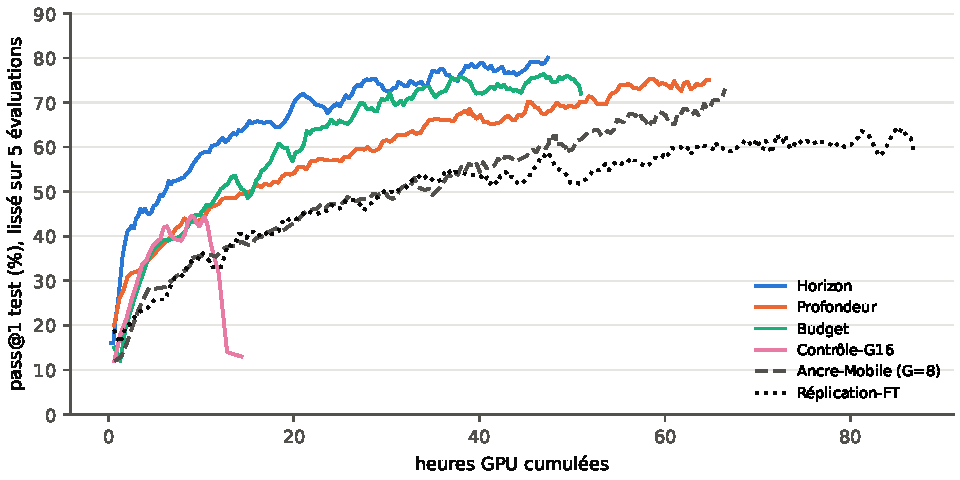
\includegraphics[width=\textwidth]{fig_pass1_gpuhours.pdf}
\column{0.5\textwidth}
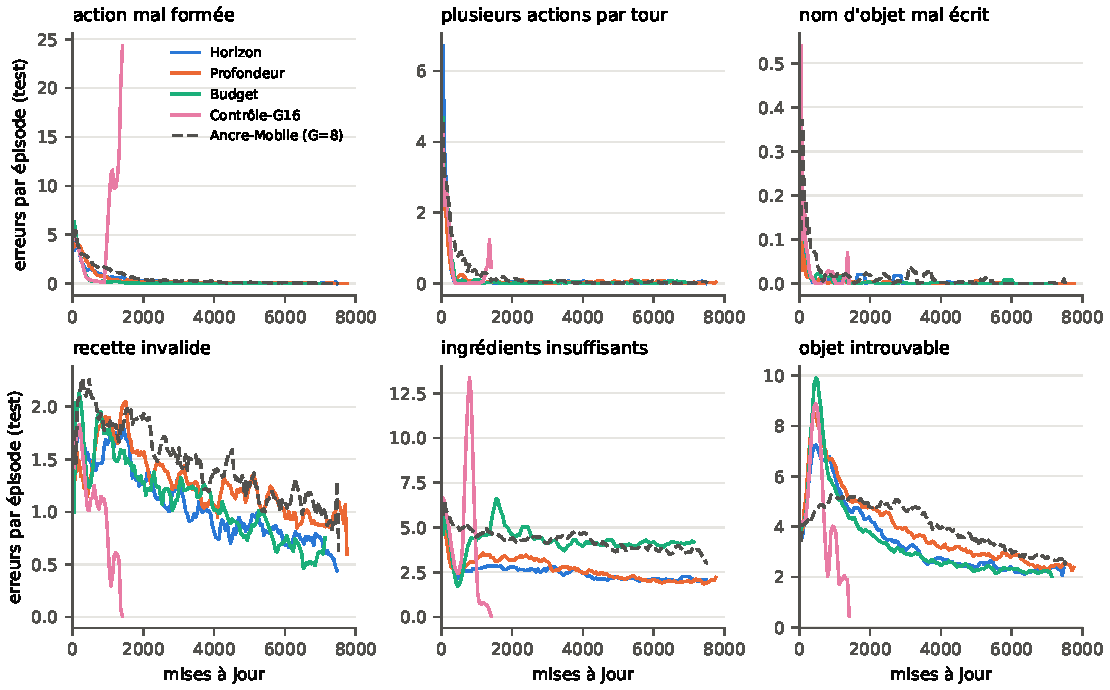
\includegraphics[width=\textwidth]{fig_errors_by_type.pdf}
\end{columns}
\vspace{0.1cm}
{\footnotesize Left: pass@1 against GPU hours per lineage. Right: error classes per run.}
\end{frame}

\begin{frame}{B10. Report figures: tokens, and control vs. curricula}
\begin{columns}[T]
\column{0.5\textwidth}
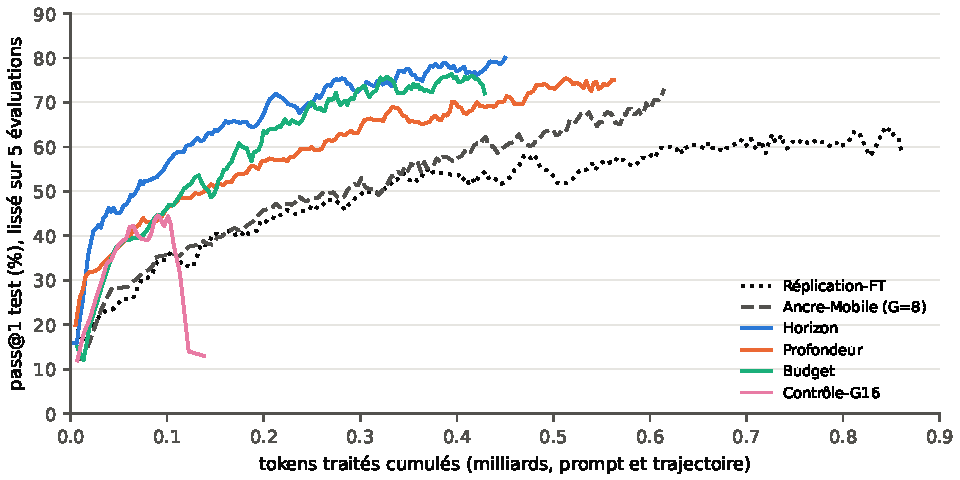
\includegraphics[width=\textwidth]{fig_pass1_tokens.pdf}
\column{0.5\textwidth}
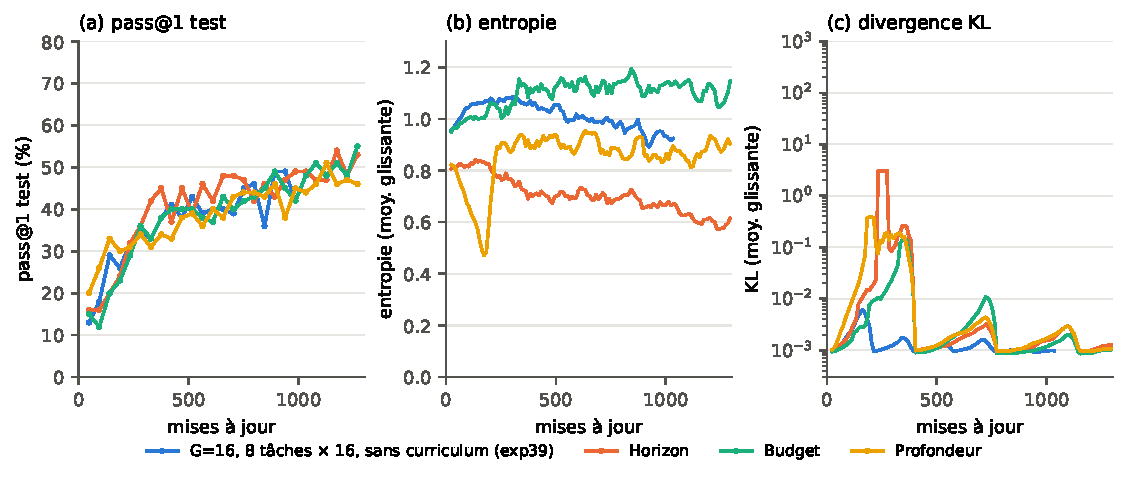
\includegraphics[width=\textwidth]{fig_exp39_vs_curricula.pdf}
\end{columns}
\vspace{0.1cm}
{\footnotesize Left: pass@1 against generated tokens. Right: the stable $G=16$ control (exp39) against the three curricula.}
\end{frame}

\begin{frame}{B11. Sixteen runs: episode length, turns, tokens per turn}
\begin{center}
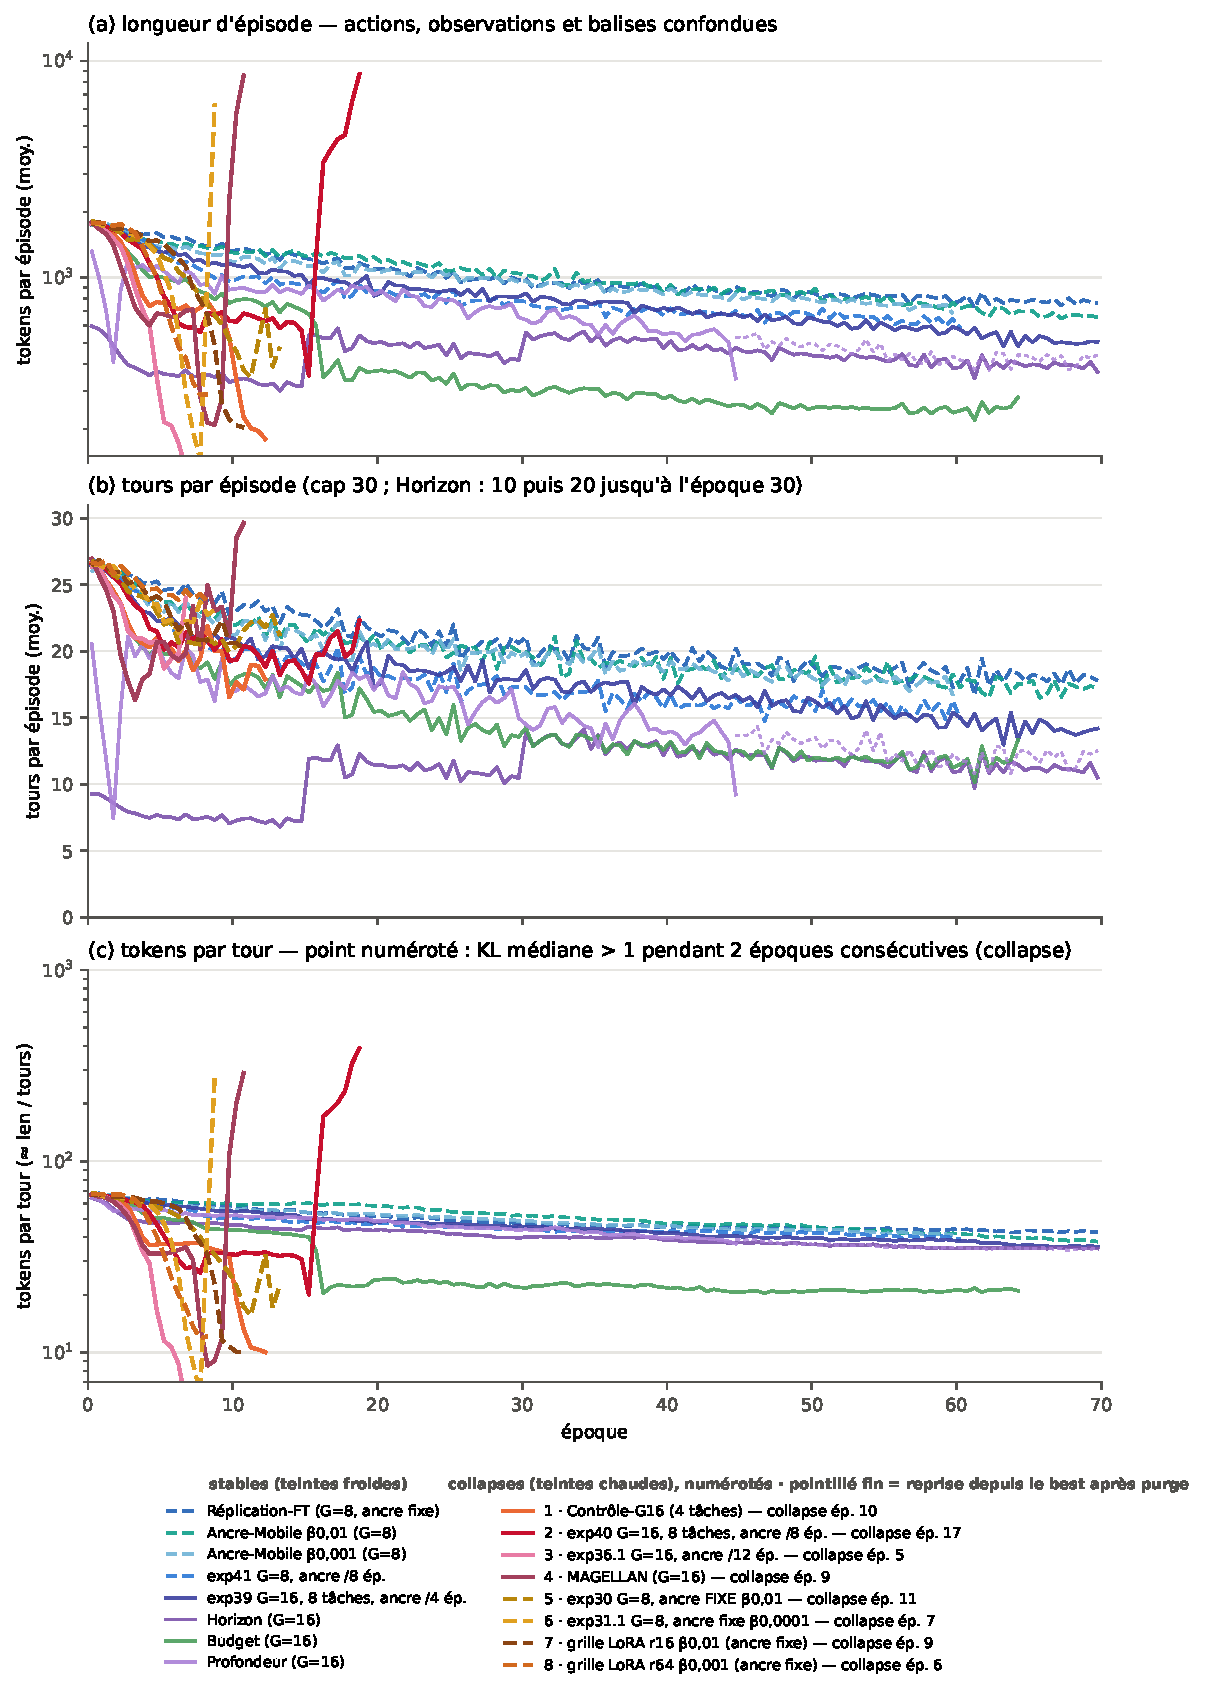
\includegraphics[height=0.78\textheight]{fig_collapse_lengths_all.pdf}
\end{center}
\end{frame}

\end{document}
